\documentclass[sigconf]{acmart}

\usepackage{xspace}
\usepackage{listings}
\usepackage{amsthm}
\usepackage{algorithm}
\usepackage{algorithmic}
\usepackage{multirow}
\usepackage{colortbl}
\usepackage{enumitem}

% TAPS-safe replacement for mdframed
\usepackage{framed}

\usepackage{tikz}
\usetikzlibrary{arrows.meta, positioning, fit, backgrounds, calc}

\newcommand{\gfaz}{GFAz\xspace}
\newcommand{\NoBcBestCr}[1]{\cellcolor{blue!15}{#1}}
\newcommand{\SecondbestCr}[1]{\cellcolor{green!15}{#1}}
\newcommand{\thiswork}{\gfaz}

\newtheorem{example}{Example}
\usepackage{acmart-taps}

\floatstyle{plain}
\newfloat{workedexample}{t}{loe}
\floatname{workedexample}{Worked Example}

\newenvironment{exampleframe}
  {\begin{framed}\noindent}
  {\end{framed}}

\lstset{
  basicstyle=\small\ttfamily,
  breaklines=true,
  frame=single,
  numbers=none,
  xleftmargin=2em,
  framexleftmargin=1.5em
}

\AtBeginDocument{%
  \providecommand\BibTeX{{%
    Bib\TeX}}}

\copyrightyear{2026}
\acmYear{2026}
\setcopyright{cc}
\setcctype{by}
\acmConference[ICS '26]{2026 International Conference on Supercomputing}{July 06--09, 2026}{Belfast, United Kingdom}
\acmBooktitle{2026 International Conference on Supercomputing (ICS '26), July 06--09, 2026, Belfast, United Kingdom}
\acmDOI{10.1145/3797905.3807870}
\acmISBN{979-8-4007-2522-7/2026/07}

%% end of the preamble, start of the body of the document source.
\begin{document}

%%
%% The "title" command has an optional parameter,
%% allowing the author to define a "short title" to be used in page headers.
\title{\gfaz: Order-of-Magnitude Pangenome Analytics by Computing over Compression}

\author{Taolue Yang}
\email{taolue.yang@temple.edu}
\orcid{0009-0000-6358-2982}
\affiliation{%
  \institution{Temple University}
  \city{Philadelphia}
  \state{PA}
  \country{USA}
}

\author{Youyuan Liu}
\email{youyuan.liu@temple.edu}
\affiliation{%
  \institution{Temple University}
  \city{Philadelphia}
  \state{PA}
  \country{USA}
}

\author{Bo Jiang}
\email{bo.jiang@temple.edu}
\affiliation{%
  \institution{Temple University}
  \city{Philadelphia}
  \state{PA}
  \country{USA}
}

\author{Xinghua Shi}
\email{mindyshi@temple.edu}
\affiliation{%
  \institution{Temple University}
  \city{Philadelphia}
  \state{PA}
  \country{USA}
}

\author{Sian Jin}
\email{sian.jin@temple.edu}
\affiliation{%
  \institution{Temple University}
  \city{Philadelphia}
  \state{PA}
  \country{USA}
}



\begin{abstract}
  Pangenome graphs stored in the Graphical Fragment Assembly (GFA) format can reach hundreds of gigabytes, with traversal records accounting for over 90\% of the file size. General-purpose compressors fail to exploit cross-haplotype redundancy in these traversals, and existing specialized tools either sacrifice full semantics or offer limited throughput, while still trailing our method in compression ratio.
  We present \gfaz, a lossless GFA compressor that compresses and decompresses in linear time. \gfaz uses iterative 2-mer grammar compression to collapse traversal redundancy, combined with columnar, type-specific encoding of all GFA record types including optional fields. Both compression and decompression are fully parallel, with a CPU backend (OpenMP) and a GPU backend (CUDA/nvComp). Across six datasets ranging from 113\,MB to 369\,GB, \gfaz achieves 18--84$\times$ compression, outperforming all evaluated baselines in compression ratio, compression throughput, and decompression throughput. The CPU backend sustains up to 385\,MB/s compression and 1.8\,GB/s decompression; the GPU backend reaches up to 4.8\,GB/s and 9.4\,GB/s, respectively.
\end{abstract}

%%
%% The code below is generated by the tool at http://dl.acm.org/ccs.cfm.
%% Please copy and paste the code instead of the example below.
%%
\begin{CCSXML}
  <ccs2012>
  <concept>
  <concept_id>10003752.10003809.10010031.10002975</concept_id>
  <concept_desc>Theory of computation~Data compression</concept_desc>
  <concept_significance>500</concept_significance>
  </concept>
  </ccs2012>
\end{CCSXML}

\ccsdesc[500]{Theory of computation~Data compression}
\ccsdesc[300]{Applied computing~Bioinformatics}
\ccsdesc[300]{Computing methodologies~Parallel algorithms}

\keywords{Biological Data Compression, Graphical Fragment Assembly}

\maketitle

\section{Introduction}\label{sec:intro}

Human genomes vary across individuals at many scales, from small variants to large structural changes, yet most analysis still relies predominantly on mapping sequencing reads to a single linear reference genome. While effective in conserved regions, this paradigm breaks down in highly polymorphic loci and in sequences absent from the reference, leading to systematic reference bias~\cite{lin2024measuring}. Pangenome graphs~\cite{eizenga2020pangenome, secomandi2025pangenome} address this limitation by representing population variation explicitly within a unified structure: nodes encode DNA segments, edges capture admissible adjacencies, and paths represent individual haplotypes. By eliminating reliance on a single reference, graph-based representations substantially improve downstream analyses, including up to 34\% fewer small-variant errors and more than doubling structural-variant discovery compared to linear-reference approaches~\cite{liao2023draft}.

Recently, the Graphical Fragment Assembly (GFA) format~\cite{gfaspec} has emerged as the de facto interchange format for pangenome graphs. GFA is simple, human-readable, and widely adopted by graph construction and analysis pipelines such as Minigraph-Cactus~\cite{hickey2024pangenome} and PGGB~\cite{garrison2024building}. However, this generality of GFA comes at a cost of scale. While graph topology grows sublinearly as haplotypes are added, traversal records grow nearly linearly because each traversal is materialized explicitly. This structural redundancy rapidly dominates file size, making large GFA files expensive to store, transfer, and process, and thus motivating the need for effective file compression.

Real pangenome datasets make this bottleneck explicit. Sirén and Paten~\cite{siren2022gbz} report that 90-haplotype human pangenome graphs constructed from year-1 HPRC data require 44.9\,GiB and 88.6\,GiB as uncompressed GFA text for Cactus and PGGB, respectively; even after gzip compression, they remain 11.1\,GiB and 14.6\,GiB. At larger cohort scale, their 5008-haplotype 1000GP graph reaches 9534.9\,GiB uncompressed and 2231.3\,GiB after gzip compression. This growth is largely driven by traversal data: in a human chromosome 19 graph with 1{,}000 haplotypes, traversals alone account for 98.7\% of a 14\,GB GFA file~\cite{heringer2025human}.

In practice, gzip-compatible compressors such as gzip and bgzip remain widely used in bioinformatics pipelines because they are ubiquitous, stable, and interoperable with existing Unix tooling. However, pangenome graphs expose a mismatch between general-purpose compression and graph structure. Gzip-style compressors operate over local byte windows and are not designed to exploit repeated traversal structure across chromosome-scale haplotypes, leaving substantial cross-haplotype redundancy unexploited.

Two specialized approaches illustrate the current design trade-offs. GBZ~\cite{siren2022gbz} achieves weaker compression on highly collapsed regions and small graphs, and is not designed for incremental updates. In contrast, sqz~\cite{heringer2025human} preserves a text workflow but is relatively slow in practice due to its heap-based Byte Pair Encoding (BPE) design. Both approaches do not preserve all original GFA record information, such as optional fields, which limits their use as fully lossless GFA text compressors.

We thus present \gfaz, a GFA compressor that achieves state-of-the-art compression ratio and high throughput on both CPU and GPU. In summary, \gfaz makes four main contributions:

\begin{itemize}[noitemsep, topsep=2pt, leftmargin=*]
    \item \textbf{Orientation-aware grammar compression}: multi-round 2-mer grammar that exploits the canonical symmetry of forward/reverse node orientations with linear-time compression and decompression.
    \item \textbf{Columnar GFA representation}: column-oriented layout for all GFA record types with type-specific encodings, enabling individual field access without full decompression.
    \item \textbf{Incremental haplotype extension and random access}: support for adding extra haplotypes without recompressing previously compressed data, and for retrieving individual haplotypes without decompressing the full dataset.
    \item \textbf{Fully parallel CPU and GPU backends}: end-to-end parallel compression and decompression using OpenMP and CUDA, with a shared format so that data compressed on CPU can be decompressed on GPU for faster decoding.
\end{itemize}

Across large human pangenome datasets, \gfaz achieves 18--84$\times$ compression, typically over 10$\times$ better than gzip/zstd baselines. CPU throughput reaches 200--400 MB/s for compression and 2 GB/s for decompression; the GPU backend reaches up to 5 GB/s and 10 GB/s, respectively. These results make \gfaz practical for large-scale pangenome storage and transfer. We release our implementation as open source at: \href{https://github.com/babyplutokurt/GFAz}{https://github.com/babyplutokurt/GFAz}.


\section{Background}\label{sec:background}

\subsection{The GFA Format}\label{subsec:gfa-format}

GFA is a line-oriented text format for sequence graphs~\cite{gfaspec}. Biologically, a graph node represents a DNA sequence segment (often shared by many individuals), edges represent allowed adjacencies between segments, and traversals represent assembled sequences or haplotypes as ordered walks through those segments.

The node record is \textbf{S} (segment), which stores a segment identifier and its DNA sequence.
Edge records include \textbf{L} (link), \textbf{J} (jump), and \textbf{C} (containment): \textbf{L} connects oriented segments (with overlap information), \textbf{J} represents long-range connections or gaps, and \textbf{C} represents containment/nesting relationships.
Traversal records are \textbf{P} (path) and \textbf{W} (walk). Both describe an ordered, orientation-aware route through nodes, which reconstructs a longer biological sequence from graph segments. \textbf{P} is a general named traversal (often a contig or reference path), while \textbf{W} (GFA~1.1) represents haplotype walks with explicit sample, haplotype, and coordinate metadata.
\textbf{H} (header) stores file-level metadata, and optional \texttt{TAG:TYPE:VALUE} fields extend records with additional annotations.
Figure~\ref{fig:gfa_visualization} shows a visualization of a GFA file using Bandage~\cite{Wick2015Bandage}.

\begin{figure}[t]
    \centering
    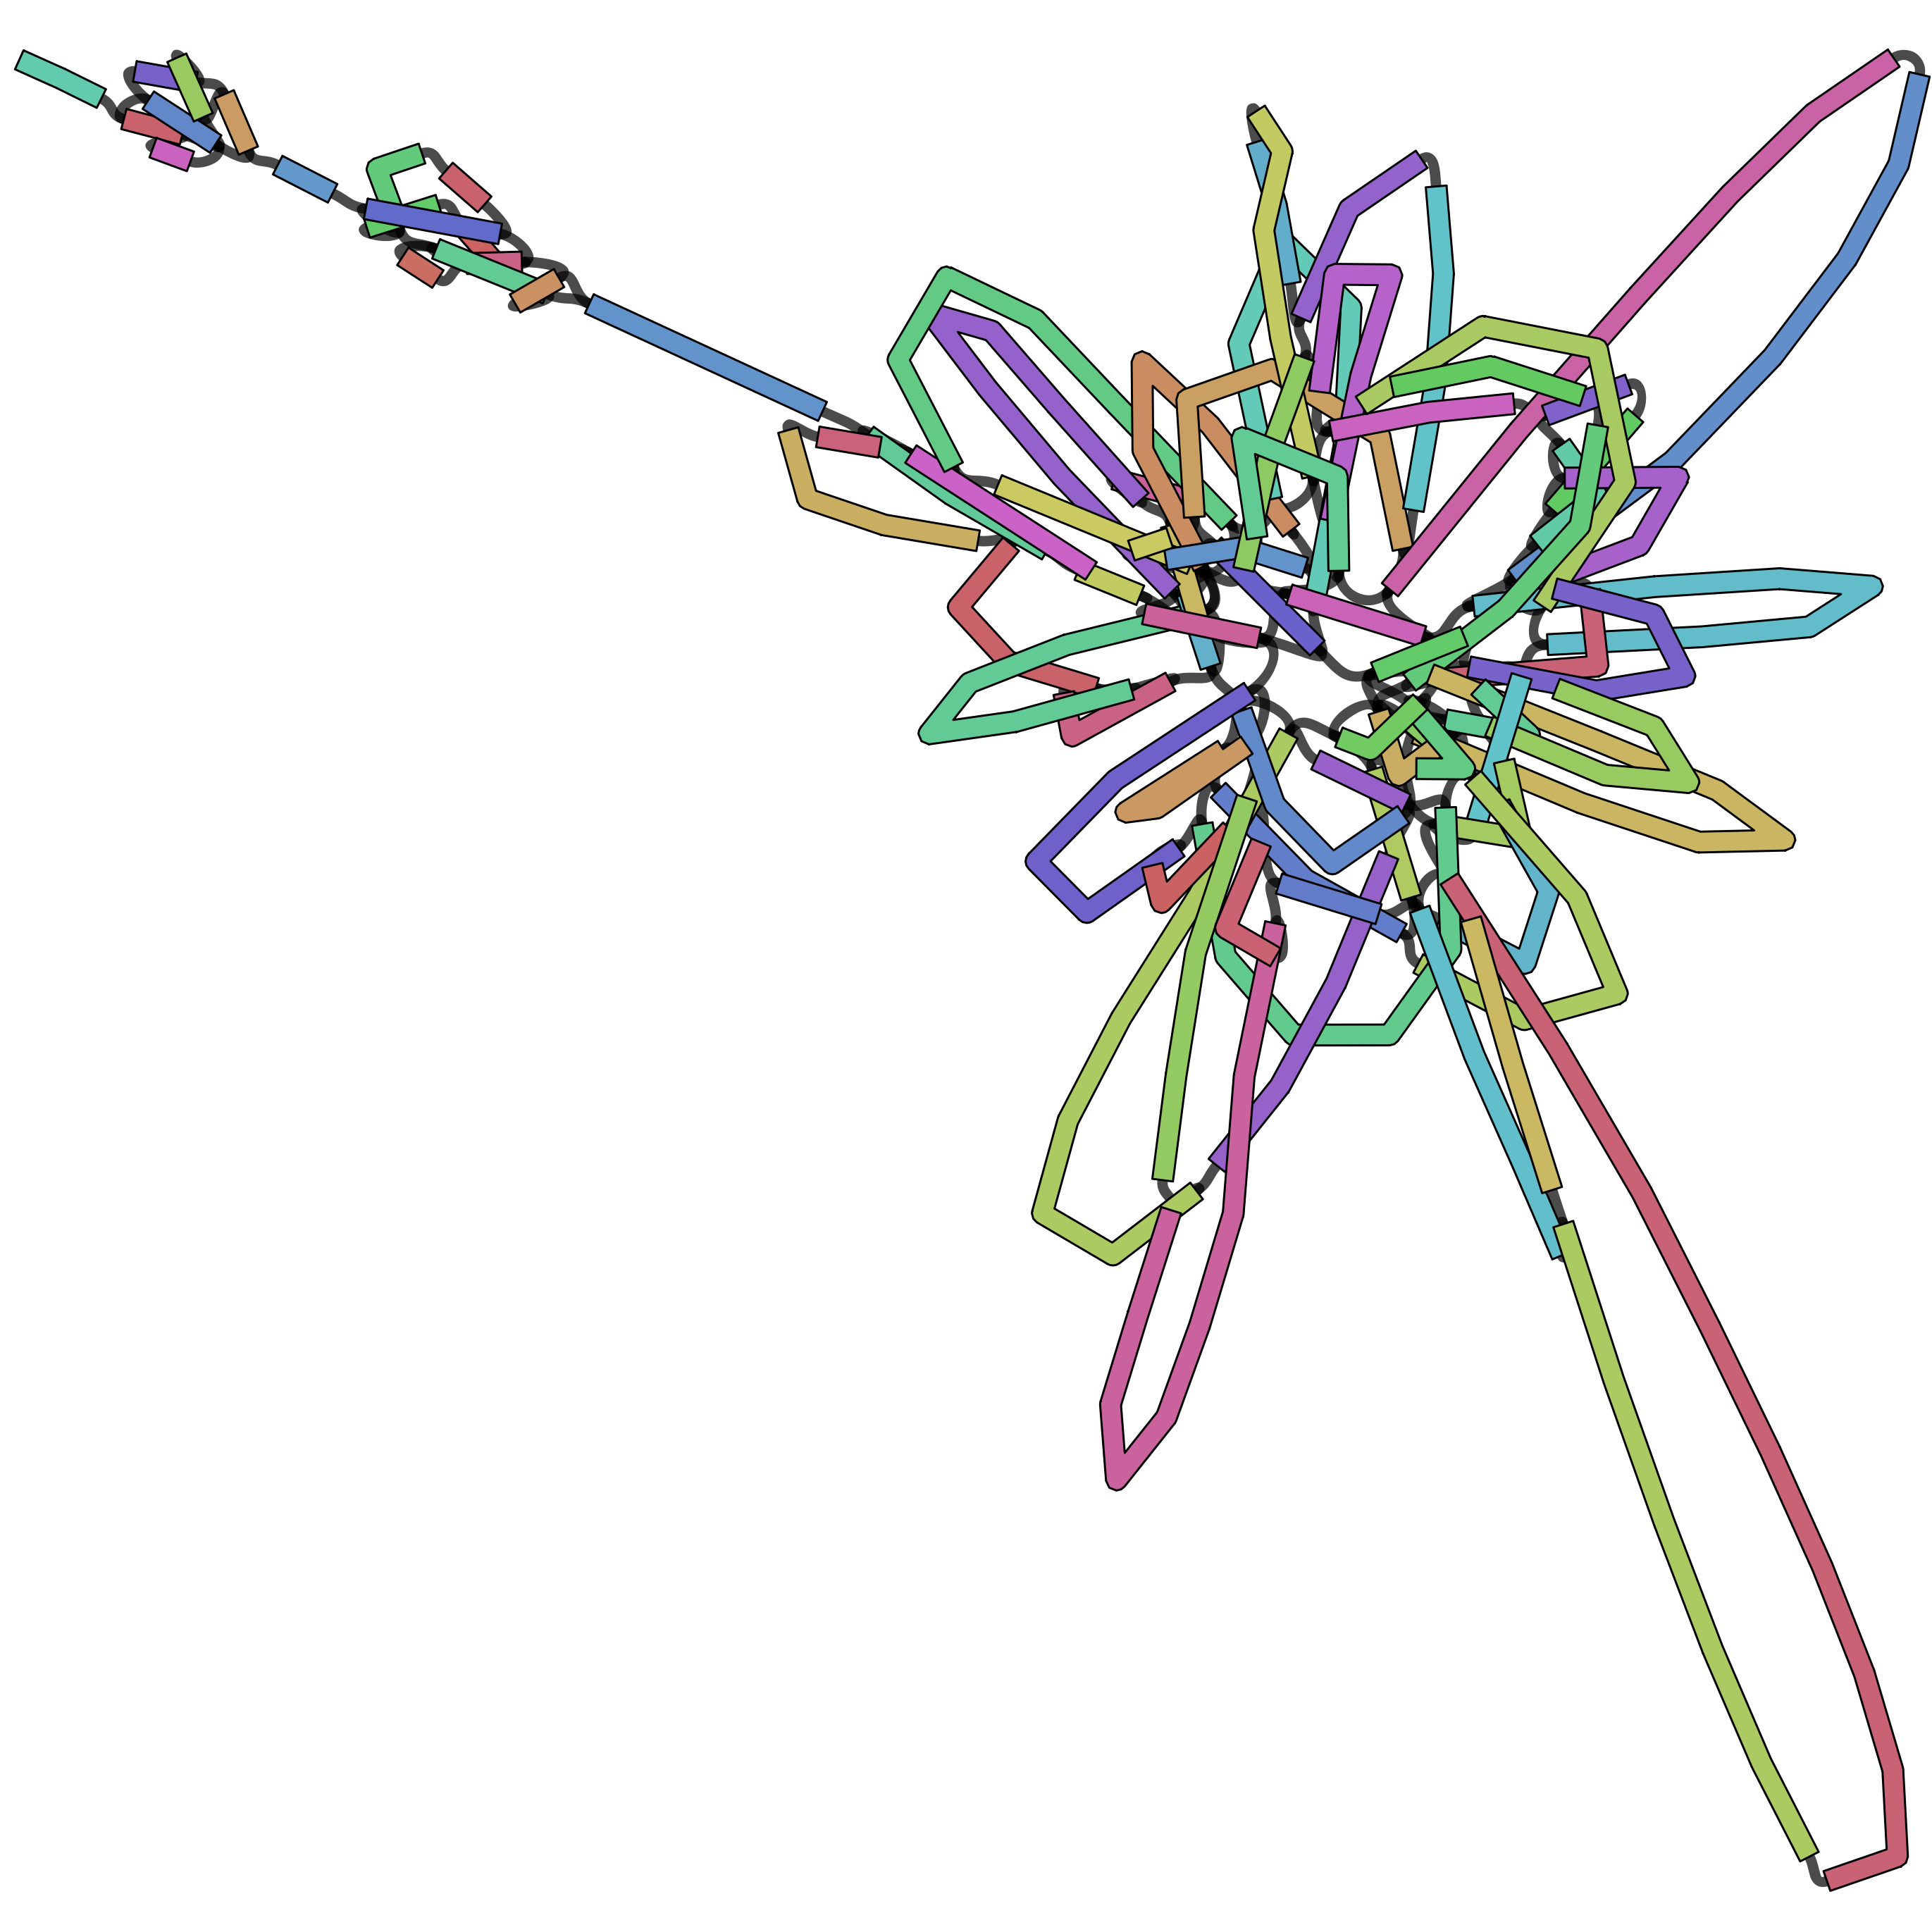
\includegraphics[width=\columnwidth]{GFA_visualization.png}
    \caption{Assembly graph in GFA format, visualized with Bandage~\cite{Wick2015Bandage}. Colored elements denote sequence segments (nodes; S records). Black connections indicate edges between oriented segments, represented by L (link), J (jump), or C (containment) records. Any valid traversal through connected segments corresponds to a P (path) or W (walk) record.}
    \label{fig:gfa_visualization}
\end{figure}

\subsection{The Scalability Challenge}\label{subsec:scalability}

GFA is widely used in graph-based genomics, including assembly graphs, pangenome construction, and downstream analysis. In pangenome graphs, shared sequence is merged into common nodes and variants form alternate branches. HPRC releases have grown from tens to hundreds of haplotypes and continue to expand~\cite{wang2022human,hprc_timeline}. Many downstream tools operate directly on GFA graphs, so these large files create both memory pressure during analysis and substantial storage overhead. At this scale, GFA becomes a systems bottleneck rather than only a storage nuisance.

As highlighted in Section~\ref{sec:intro}, real pangenome GFA files already reach very large sizes. The core scaling mechanism is structural: topology (S/L/J/C records) grows sublinearly as haplotypes are added, but traversal records (P/W) grow near-linearly because each haplotype walk is materialized explicitly. Since human haplotypes are highly similar, these long traversal streams contain substantial repeated node-ID substrings across samples. At even larger population sequencing scales, this growth will continue, pushing GFA datasets beyond hundreds gigabytes into multi-terabyte regimes. In practice, pipelines also produce many intermediate GFAs (per chromosome, per version, and per region), further amplifying storage and transfer costs.

Generic compressors cannot exploit most of this redundancy. Their small sliding windows miss long-range similarity across chromosome-length paths, so compression ratio remains limited for GFA files.

\subsection{Existing Compression Approaches}\label{subsec:existing}

Because generic compressors miss long-range path redundancy, specialized GFA compressors are needed. Other genomic compression families are also not a direct fit: read/alignment formats such as BAM/CRAM~\cite{li2009sequence, bonfield2022cram} target mapped reads rather than graph interchange files, and FASTQ compressors such as GPUFastQLZ~\cite{yang2024gpufastqlz} target linear sequence collections rather than graph topology and traversal semantics. For GFA graphs, compression must remain fully lossless to preserve graph structure and metadata while still exploiting cross-haplotype traversal redundancy.
Two graph-native approaches are GBZ and sqz.

GBZ uses Graph-Based Burrows–Wheeler Transform (GBWT)~\cite{siren2020haplotype, siren2021pangenomics} to store large collections of similar paths efficiently. This design is effective for large pangenomes with many similar haplotypes.
Its weaknesses are practical. Performance can degrade in highly collapsed repetitive regions, and compression ratio is less favorable on small graphs. Because GBWT construction is global, GBZ also does not naturally support incremental updates (e.g., appending new haplotypes) without rebuilding the index. In addition, GBZ does not preserve full GFA record semantics, like optional fields.

sqz keeps a text workflow and applies a heap-based BPE grammar design~\cite{zouhar2023formal} to path records. It repeatedly selects frequent adjacent 2-mers and replaces them with new rules.
The main limitations are speed and memory cost. After each new rule, sqz updates frequencies of affected neighboring pairs through adjacency-list bookkeeping, which makes each rule-creation step expensive in practice. This sequential dependency also limits parallelization, because each next substitution depends on the current global pair statistics. Similar to GBZ, sqz does not preserve full optional-field information, so it is not truly lossless for complete GFA records.


\section{Methodology}\label{sec:methodology}

\begin{table}[t]
  \caption{Mapping from GFA record types to \gfaz internal integer-based representation.}
  \label{tab:data-mapping}
  \small
  \begin{tabular}{lll}
    \hline
    \textbf{GFA Record} & \textbf{Graph Role} & \textbf{Internal Representation}    \\
    \hline
    S-line              & Node Definition     & \texttt{uint32\_t} (1-based ID)     \\
    L, J, C-lines       & Graph Topology      & \texttt{vector<int32\_t>{}}         \\
    P, W-lines          & Graph Traversal     & \texttt{vector<vector<int32\_t>{}>} \\
    \hline
  \end{tabular}
\end{table}

This section presents \gfaz as a modularly designed compression pipeline with two interchangeable backends: CPU (OpenMP) and GPU (CUDA/Thrust/nvComp)~\cite{nvcomp_github}. The final entropy-encoding layer is also modular, so it can be changed or tuned easily to trade compression ratio against throughput.


\subsection{Graph View of GFA}\label{subsec:graph-view}

A GFA file is a tab-delimited graph format with a small set of record types. \gfaz converts these heterogeneous text records into a compact Structure-of-Arrays layout of typed columns. Segments (S-lines) receive compact 1-based integer IDs, with sequences stored separately. Links, jumps, and containments (L/J/C-lines) become integer endpoint columns plus bit-packed orientation columns, with auxiliary strings stored as concatenated byte streams and offsets. Most importantly, both paths and walks (P/W-lines) are normalized to the same signed \texttt{int32\_t} traversal representation, where the sign encodes orientation; for example, \texttt{>s1<s2>s3} becomes \texttt{[1, -2, 3]}. This conversion turns verbose GFA text into compressible integer and byte streams, with traversals forming the dominant input to the grammar-compression pipeline.

Table~\ref{tab:data-mapping} summarizes how the text-to-integer mapping prepares each component for the compression pipeline.



\subsection{Architecture Overview}\label{subsec:architecture}

Figure~\ref{fig:compression_workflow} and \ref{fig:decompression_workflow} show the end-to-end workflow. A GFA file is first parsed into an in-memory graph representation: on the CPU this is a \texttt{GfaGraph} with nested vectors; for the GPU backend the traversals are flattened into a single contiguous array paired with a lengths vector, with offsets computed on-demand via parallel prefix sum. The parsed graph is then compressed into a \texttt{CompressedData} object containing byte blocks for every field, and can be serialized to a binary \texttt{.gfaz} file for persistent storage. Decompression is intentionally asymmetric: fixed-width graph fields are restored from their encoded columns, but traversal records are expanded and emitted as GFA text in a streaming fashion rather than rebuilding a full in-memory \texttt{GfaGraph}.

Both compression and decompression are fully parallel at every step. As introduced above, the pipeline supports CPU and GPU execution; the GPU backend keeps traversal data device-resident throughout the compression loop, transferring only the final compressed blocks back to the host.

\begin{figure}[t]
  \centering
  
\includegraphics[width=\columnwidth]{Compression_workflow.png}
  \caption{\thiswork compression workflow. The grammar compression loop repeats for $N$ rounds (default 8); each round replaces repeated 2-mers, reducing the traversal stream by up to half.}
  \label{fig:compression_workflow}
\end{figure}




\subsection{Compression Pipeline}\label{subsec:pipeline}
The central challenge in GFA compression is traversal data (P and W records), which often exceeds 90\% of file size. Traversals are highly redundant: many haplotypes share long node-ID substrings across P-lines and W-lines.

\gfaz exploits this structure with iterative grammar compression. In each round, we find frequent adjacent 2-mers (initially node IDs), assign each 2-mer a new integer ID, and replace all occurrences. Later rounds can combine original nodes with rule IDs, or combine rule IDs with each other. This hierarchy collapses long repeated patterns into single symbols and sharply reduces traversal length.

\noindent \textbf{Rule Definition.}
We formally define a \emph{rule} as a new unique integer identifier assigned to a repeated 2-mer. Like segment IDs, rule IDs are signed 32-bit integers where the sign encodes orientation. If a rule $r$ ($r > 0$) represents the 2-mer $(u, v)$, then its negation $-r$ represents the reverse complement 2-mer $(-v, -u)$. This symmetry stems from the fact that traversing a subgraph in reverse flips the order and orientation of all constituents.
\begin{equation}
  r \Rightarrow (u, v) \quad \iff \quad -r \Rightarrow (-v, -u)
\end{equation}
By treating rules as oriented symbols identical in format to node IDs, the compression engine can recursively combine nodes and rules without special cases.

\begin{algorithm}[t]
  \caption{\thiswork Compression Pipeline}
  \label{alg:compression}
  \begin{algorithmic}[1]
    \REQUIRE GFA file $F$, rounds $R$, delta\_rounds $D$
    \ENSURE Compressed data $C$
    \STATE $G \gets \text{Parse}(F)$
    \FOR{$i = 1$ to $D$}
    \STATE $\text{DeltaTransform}(G.\text{paths})$
    \STATE $\text{DeltaTransform}(G.\text{walks})$
    \ENDFOR
    \STATE $\text{next\_id} \gets \max(\text{MaxAbs}(G.\text{paths}), |G.\text{segments}|) + 1$
    \FOR{$r = 1$ to $R$}
    \STATE $\text{rules} \gets \text{GenerateRules}(G.\text{paths}, G.\text{walks})$
    \STATE $\text{EncodePaths}(G.\text{paths}, G.\text{walks}, \text{rules})$
    \STATE $\text{CompactSortRemap}(\text{rules}, G.\text{paths}, G.\text{walks})$
    \ENDFOR
    \STATE $C \gets \text{CompressAllFields}(G, \text{rules})$
    \RETURN $C$
  \end{algorithmic}
\end{algorithm}

\subsubsection{Phase 1: Delta Encoding and Rule Namespace Allocation}

We begin traversal compression with a single delta-encoding pass. For a sequence $[n_1, n_2, \ldots, n_k]$, we produce $[n_1, n_2 - n_1, n_3 - n_2, \ldots, n_k - n_{k-1}]$ and then run grammar compression on this transformed stream.
This step is effective because pangenome graph builders often assign segment IDs in approximate reference order. Many haplotypes therefore contain long runs of locally consecutive IDs, and one delta pass collapses these runs into short repeated differences. For \gfaz, the main benefit is not merely smaller values, but a much smaller adjacent-pair space for rule mining: many distinct 2-mers in the original traversal stream become the same few repeated 2-mers after delta encoding. Table~\ref{tab:delta-rounds} shows this effect on a chromosome-scale graph: one delta pass reduces the first-round rule search space by over $25\times$ and gives the best final size.

\begin{table}[t]
  \caption{Effect of delta encoding rounds on rule search space and final traversal size for \texttt{chr6.pan.gfa} (human chromosome~6 pangenome GFA). All results use 8 grammar-compression rounds.}
  \label{tab:delta-rounds}
  \small
  \begin{tabular}{lrrr}
    \hline
    \textbf{Delta rounds} & \textbf{Rules (round 1)} & \textbf{Total rules} & \textbf{Final size} \\
    \hline
    0                     & 5{,}455{,}923            & 29{,}391{,}077       & 3.60\%              \\
    1                     & 201{,}503                & 6{,}124{,}767        & 2.88\%              \\
    2                     & 264{,}485                & 6{,}281{,}692        & 2.99\%              \\
    3                     & 372{,}451                & 7{,}053{,}633        & 3.11\%              \\
    \hline
  \end{tabular}
\end{table}

We therefore use exactly one delta pass throughout the system. Additional delta rounds do not improve compression ratio, because later rule IDs no longer preserve the sequential locality of original segment IDs.

To separate literals from grammar rules, we reserve the rule namespace above all literal values. We set the starting ID to:
\begin{equation}
  I_{start} = \max\left(\max_{p \in \mathcal{P}} \max_{v \in p} |v|, \, |S|\right) + 1
\end{equation}
where the first term covers all values in the delta-encoded streams and $|S|$ covers valid segment IDs. This guarantees that a single check ($|x| \ge I_{start}$) uniquely identifies a rule.

\subsubsection{Phase 2: Hierarchical 2-Mer Grammar Compression}

The engine of our pipeline is a multi-round algorithm that recursively replaces frequent 2-mers with the rule IDs defined in the previous section. A \emph{2-mer} in this context is simply an ordered pair of signed integers $(u, v)$, representing adjacent elements in a traversal.

Since GFA paths represent double-stranded DNA, a traversal $(u, v)$ and its reverse complement $(-v, -u)$ should map to the same rule. We therefore normalize every observed 2-mer to a \emph{canonical form} by selecting the lexicographically smaller of its forward and reverse representations.
\begin{equation}
  \text{pack}(u, v) = ((int64)u \ll 32) \mid (v \ \& \ \texttt{0xFFFFFFFF})
\end{equation}
\begin{equation}
  \text{canonical}(u, v) = \min\left(\text{pack}(u, v), \text{pack}(-v, -u)\right)
\end{equation}
By hashing and counting only these canonical values, occurrences on either strand contribute to the same rule. Each rule therefore corresponds to exactly one canonical 2-mer, while the sign of the emitted rule ID records whether the observed occurrence matches the canonical orientation or its reverse.

\noindent \textbf{Rule Generation.} To identify 2-mers that appear at least twice, we use a parallel ``two-set'' strategy that avoids building a full frequency table. Each thread scans adjacent pairs, inserts first occurrences into a local \emph{seen} set, and promotes second occurrences to a local \emph{repeated} set. The thread-local sets are then reduced into global \emph{seen} and \emph{repeated} sets, so a 2-mer observed once in multiple threads is still promoted to \emph{repeated}. Paths and walks are processed together in this pass, ensuring that a 2-mer appearing once in a path and once in a walk is still detected as repeated. Finally, we assign sequential rule IDs to the unique canonical 2-mers in the global \emph{repeated} set.

Suppose $n$ unique repeated 2-mers are found. Each is assigned a rule ID sequentially: the first receives $\text{start\_id}$, the second $\text{start\_id} + 1$, and so on up to $\text{start\_id} + n - 1$. Two structures are built: a hash map from canonical 2-mer to rule ID for $O(1)$ lookup during encoding, and a vector of length $n$ indexed by $(\text{rule\_id} - \text{start\_id})$ for $O(1)$ reverse lookup during later expansion.

\noindent \textbf{Traversal Encoding and Rule Tracking.}
We encode each traversal by scanning left-to-right, checking every consecutive 2-mer against the rule hash map. For each 2-mer $(u, v)$, we first check if its canonical form corresponds to a known rule ID $r$. If so, we check orientation: if $(u, v)$ matches the canonical order, we replace the 2-mer with $+r$; if it matches the reverse complement order $(-v, -u)$, we replace it with $-r$.

Because rules are generated from the pre-encoding stream, newly emitted rule IDs cannot participate in additional same-round matches, so encoding remains a simple left-to-right scan.

During this process, we maintain a usage bitmap, \texttt{rules\_used}, to track which generated rules are actually applied. This is necessary because greedy substitution may leave some generated rules unused; whenever a rule $r$ is emitted, we set $\texttt{rules\_used}[|r| - \text{start\_id}] = 1$.


\begin{table}[t]
  \centering
  \caption{Internal columnar data structures for each GFA record type before final ZSTD compression.}
  \label{tab:columnar-structures}
  \resizebox{\columnwidth}{!}{%
    \begin{tabular}{lll}
      \toprule
      \textbf{GFA Record}                        & \textbf{Component Fields} & \textbf{Internal Data Structure}                                    \\
      \midrule
      \multirow{2}{*}{\textbf{Rules}}            & Dictionary (First/Second) & Two parallel \texttt{vector<int32\_t>}                              \\
                                                 & Layer Ranges              & \texttt{vector<LayerRuleRange>}                                     \\ \cline{2-3}

      \multirow{2}{*}{\textbf{Segments (S)}}     & Sequences                 & Concatenated \texttt{string} + Lengths (\texttt{vector<uint32\_t>}) \\
                                                 & Optional Fields           & Type-specific columns (varint, float, string)                       \\ \midrule

      \multirow{4}{*}{\textbf{Links (L)}}        & From/To Node IDs          & Parallel \texttt{vector<uint32\_t>}                                 \\
                                                 & Orientations              & Bit-packed \texttt{vector<uint8\_t>} (1 bit/edge)                   \\
                                                 & Overlaps                  & Parallel \texttt{vector<uint32\_t>} / \texttt{vector<char>}         \\
                                                 & Optional Fields           & Type-specific columns                                               \\ \midrule

      \multirow{4}{*}{\textbf{Jumps (J)}}        & From/To Node IDs          & Parallel \texttt{vector<uint32\_t>} (delta+varint)                  \\
                                                 & Orientations              & Bit-packed \texttt{vector<uint8\_t>}                                \\
                                                 & Distance                  & Concatenated \texttt{string} + Lengths                              \\
                                                 & Rest Fields               & Concatenated \texttt{string} + Lengths                              \\ \midrule

      \multirow{5}{*}{\textbf{Containments (C)}} & Container/Contained IDs   & Parallel \texttt{vector<uint32\_t>} (delta+varint)                  \\
                                                 & Orientations              & Bit-packed \texttt{vector<uint8\_t>}                                \\
                                                 & Position                  & \texttt{vector<uint32\_t>} (ZSTD)                                   \\
                                                 & Overlap (CIGAR)           & Concatenated \texttt{string} + Lengths                              \\
                                                 & Rest Fields               & Concatenated \texttt{string} + Lengths                              \\ \midrule

      \multirow{3}{*}{\textbf{Paths (P)}}        & Encoded Sequence          & Flattened \texttt{vector<int32\_t>} (Rules/IDs)                     \\
                                                 & Path Names, Overlaps      & Concatenated \texttt{string} + Lengths                              \\
                                                 & Path Lengths              & \texttt{vector<uint32\_t>} (Original \& Compressed)                 \\ \midrule

      \multirow{4}{*}{\textbf{Walks (W)}}        & Encoded Sequence          & Flattened \texttt{vector<int32\_t>} (Rules/IDs)                     \\
                                                 & Sample/Seq IDs            & Concatenated \texttt{string} + Lengths                              \\
                                                 & Haplotype/Start/End       & \texttt{vector<uint32\_t>} + \texttt{vector<int64\_t>} (varint)     \\
                                                 & Walk Lengths              & \texttt{vector<uint32\_t>}                                          \\
      \bottomrule
    \end{tabular}%
  }
\end{table}


\noindent \textbf{Compact, Sort, and Remap.}
After encoding, we optimize the rule set for storage and the next grammar round via three fused operations:
\begin{enumerate}[noitemsep, topsep=2pt, leftmargin=*]
  \item \textbf{Compact (Prune Unused):} As noted, greedy encoding leaves gaps in the rule index space. To remove them, we perform an \emph{exclusive prefix sum} on the \texttt{rules\_used} bitmap. The result at index $i$ gives the exact destination index for the rule at $(\text{start\_id} + i)$ in the new particular array. For example, if \texttt{rules\_used} is $[1, 0, 1, 1]$, the prefix sum is $[0, 1, 1, 2]$. This tells us: rule $0$ moves to pos $0$, rule $1$ is skipped, rule $2$ moves to pos $1$, and rule $3$ moves to pos $2$. We then gather only the active rules into a value-contiguous array using these computed offsets, completely eliminating gaps in parallel.

  \item \textbf{Sort (Optimize Layout):} We sort all the active rules by their packed 2-mer content. This step is crucial for the compression of the rulebook itself. By ordering rules lexicographically (primarily by their first element $u$, secondarily by $v$), we cluster rules that share the same starting node. For storage, each packed 64-bit rule key is split into its upper 32 bits and lower 32 bits. After sorting, the upper-32-bit stream becomes highly repetitive (e.g., $[\ldots, u, u, u, w, w, \ldots]$), so delta encoding produces long zero runs and sharply reduces rulebook size.


  \item \textbf{Remap (Update Streams):} Finally, we assign permanent, sequential IDs to the rules in their new sorted order, starting from the current global \texttt{next\_id}. We verify the permutation by building a lookup table, $T[\text{old\_id} - \text{range\_start}] = \text{new\_id}$. A parallel function then sweeps over all paths: any element $e$ falling in the current round's range is updated to $T[|e| - \text{range\_start}]$ (preserving the original sign). Upon completion, we update \texttt{start\_id} to be the last assigned rule ID $+ 1$, ensuring that rules in the next grammar round begin exactly where the current set ends, which results in sequential rule IDs across all rounds, ranging from the first round's start ID to the last end ID.
\end{enumerate}

The Generation-Encoding-Compact, Sort and Remap phases constitute a single round. We repeat this process iteratively (typically 8 times). As described earlier, subsequent rounds can pair the rules created in previous steps, allowing the algorithm to capture exponentially longer patterns (length 4, 8, 16, and beyond) and recursively collapse long repetitive haplotype blocks into single rule IDs.
After these rounds, the traversal data consists of encoded traversal streams, a global rulebook stored as parallel \texttt{rules\_first} and \texttt{rules\_second} vectors, and the boundary value \texttt{start\_id} that separates literals from rule IDs during decoding. This representation exposes both traversals and rules as integer streams for the final field-specific encoding phase.

\subsubsection{Phase 3: Field-Specific Encoding}

After Phases 1--2, \gfaz stores the graph as typed streams. Phase 3 converts all records to a columnar Structure-of-Arrays (SoA) layout: one contiguous column per field. Each column then uses a type-specific encoder:

\begin{itemize}[noitemsep, topsep=2pt, leftmargin=*]
  \item \textbf{Integers (IDs, lengths, positions)}: Near-monotonic ID columns (e.g., link/jump/containment endpoints) use delta + varint. Other fixed-width integer columns use dense arrays + ZSTD. Rule columns use delta + ZSTD.
  \item \textbf{Booleans (orientations)}: Bit-packed (8 values/byte), up to $8\times$ smaller than byte-per-flag storage.
  \item \textbf{Strings (names, DNA, CIGARs, auxiliary fields)}: Concatenated byte streams with offset arrays, then ZSTD.
\end{itemize}


\begin{figure}[t]
  \centering
  
\includegraphics[width=\columnwidth]{Decompression_workflow.png}
  \caption{\thiswork decompression workflow. Traversal expansion runs in linear time and is dependency-free across records, enabling batched parallel decode and direct streaming output without rebuilding the full graph in memory.}
  \label{fig:decompression_workflow}
\end{figure}





\noindent \textbf{Optional Fields.}
(\texttt{TAG:TYPE:VALUE}) are encoded by \texttt{TYPE}:
\begin{itemize}[noitemsep, topsep=2pt, leftmargin=*]
  \item \texttt{i} (integer): varint-encoded vector.
  \item \texttt{f} (float): float vector.
  \item \texttt{A} (character): contiguous byte array.
  \item \texttt{Z} (string), \texttt{J} (JSON), \texttt{H} (hex): concatenated stream with offsets.
  \item \texttt{B} (numeric array): flattened value stream (subtype-dependent, e.g., \texttt{c,s,i,f}) + per-row length vector.
\end{itemize}




Sparse optional fields are handled by sentinel padding: if the $N$-th record lacks a tag, we insert a sentinel value into that column. This preserves $O(1)$ indexing, and the resulting runs of identical sentinels compress effectively under ZSTD.

Table~\ref{tab:columnar-structures} lists the specific columnar structures used for each GFA component.




\subsubsection{Phase 4: ZSTD Compression}

All encoded fields are finally compressed with ZSTD~\cite{collet2021rfc}. By this stage, the dominant data (traversals) has already been aggressively reduced by grammar compression and type-specific encoding, so ZSTD operates mostly on compact, low-entropy streams. We use ZSTD at level 9 (configurable via environment variable) to balance throughput and compression ratio.





\subsection{Decompression Pipeline}\label{subsec:decompression}

Decompression is partly symmetric to compression. For segments, links, jumps, containments, and optional fields, the decoder simply applies the inverse of the field-specific encodings used in Phase~3 and Phase~4: ZSTD decompression, inverse delta, varint decoding, and orientation bit-unpacking. These field restorations are independent and run in parallel sections.

Traversal decoding is intentionally asymmetric. Rather than rebuilding a full in-memory \texttt{GfaGraph}, \gfaz expands P/W records with a streaming pipeline. The decoder directly uses \texttt{rules\_first}, \texttt{rules\_second}, and \texttt{start\_id}; no extra rulebook reconstruction step is required. Traversals are partitioned into batches, multiple threads expand and decode one batch at a time, and each batch is written directly as GFA lines to the output file. This design keeps peak memory bounded by the working batch rather than by the total size of all paths and walks.

For each encoded traversal element $e$:

\begin{enumerate}[noitemsep, topsep=2pt, leftmargin=*]
  \item \textbf{Check}: If $|e| < \text{start\_id}$, it is a literal node ID; we append it directly to the output.
  \item \textbf{Expand}: If $|e| \ge \text{start\_id}$, it is a rule. We resolve its children via direct array lookup at index $(|e| - \text{start\_id})$.
  \item \textbf{Recurse}: This lookup mimics a depth-first traversal of the grammar tree. We recursively expand the children until we reach literals. Crucially, if the rule ID $e$ is negative, we expand the children in \emph{reverse order} and flip their signs.
\end{enumerate}


\noindent After expansion, inverse delta is applied $D$ times to recover the original node IDs. The recovered oriented IDs are then converted immediately back into the textual P-line or W-line syntax and appended to the output stream. Because traversals are independent, this batched decode-and-write procedure parallelizes naturally across CPU threads. After traversal expansion, the rule table is freed to reclaim memory.
This design ensures high throughput. Rule resolution is strictly $O(1)$ (an array read), involving no hash table lookups or complex pointer chasing.



Although the CPU and GPU backends may produce different rule sets and encoded traversal streams, both serialize into the same format (\texttt{rulebook + start\_id + encoded traversals}), so either backend can correctly decompress files produced by the other.

\subsection{Incremental Haplotype Extension and Random Access}\label{subsec:random-access}

\gfaz supports random access to individual haplotypes and incremental extension by appending new haplotypes. Both operations decode only the lightweight traversal vectors, metadata columns, and stored grammar rules, without reprocessing the full graph.

\noindent \textbf{Random Access.}
The \texttt{extract-traversal} operation reconstructs only the requested haplotype. \gfaz locates the target path or walk from its metadata columns, slices the corresponding encoded subsequence from the flattened traversal vector, expands the grammar rules, applies inverse delta decoding, and emits only that record.

\noindent \textbf{Incremental Extension.}
The \texttt{add-haplotypes} operation appends new paths or walks using the rulebook already stored in the input \texttt{.gfaz} file. \gfaz validates the new haplotypes, applies the delta transform, encodes only the appended paths or walks, and writes back the updated columns.
To preserve decodability, the appended traversal values must remain outside the rule-ID range. Let \texttt{start\_id} denote the first rule ID stored in the existing file. \gfaz verifies that the maximum delta value in the appended traversals is smaller than \texttt{start\_id}, ensuring that these literals cannot be misinterpreted as grammar rules during later decoding.

\subsection{GPU Backend}\label{subsec:gpu}

\gfaz implements a high-performance GPU backend designed to keep the \emph{traversal compression loop} device-resident. After transferring the traversal stream to GPU memory, all per-round operations---2-mer mining, rule table construction, parallel rule application, and stream compaction---execute on the GPU, avoiding the CPU-side dependency chain that constrains the serial greedy algorithm.

\noindent \textbf{Parallel 2-mer Mining via Sorting.}
The most computationally intensive step is identifying repeated 2-mers. Traditional hash-counting is unsuitable for the GPU due to atomic contention. Instead, we implement a dependency-free, sort-based pipeline given a vector of node IDs $D$ of length $N$:
\begin{enumerate}[noitemsep, topsep=2pt, leftmargin=*]
  \item \textbf{\textsc{GenerateKeys} (Canonical 2-mer Keys)}: Since the input size $N$ is known, we allocate a device vector of size $M=N-1$. A massively parallel kernel launches one thread per index $i \in [0, M)$ and writes a canonical packed 2-mer:
        \[
          K_i = \min(\text{pack}(D_i, D_{i+1}), \text{pack}(-D_{i+1}, -D_i)).
        \]
        This step is embarrassingly parallel and requires no synchronization.
  \item \textbf{\textsc{SortKeys} (Group Identicals)}: We sort $K$ on the GPU (radix sort) so that identical 2-mers form contiguous runs.
  \item \textbf{\textsc{MarkDuplicates} (Run Membership)}: In parallel, we compute a boolean flag $F_i$ that marks whether $K_i$ belongs to a run, using only neighbor comparisons:
        \[
          F_i =
          \begin{cases}
            (K_0 = K_1),                             & i=0,     \\
            (K_i = K_{i-1}) \ \vee\ (K_i = K_{i+1}), & 0<i<M-1, \\
            (K_{M-1} = K_{M-2}),                     & i=M-1.
          \end{cases}
        \]
  \item \textbf{\textsc{CompactUnique} (Extract Repeats)}: We apply stream compaction (\texttt{copy\_if}) to extract all keys with $F_i=1$, then apply \texttt{unique} to produce the final set of repeated 2-mers (frequency $\ge 2$) used as candidate rules for this round.
\end{enumerate}




\begin{algorithm}[t]
  \caption{GPU Parallel 2-mer Mining}
  \label{alg:gpu-mining}
  \begin{algorithmic}[1]
    \STATE \textbf{Input:} Device vector $D$ (int32 nodes), integer $N$
    \STATE \textbf{Output:} Device vector $Repeats$ (unique int64 2-mers)

    \STATE $M \gets N-1$
    \STATE $Keys \gets$ \textbf{ALLOCATE\_DEVICE\_VECTOR}($M$)

    \STATE \COMMENT{1. \textsc{GenerateKeys}: canonical packed 2-mers}
    \STATE \textbf{PARALLEL\_FOR} $i \in \{0 \dots M-1\}$
    \STATE \hspace{0.6cm} $K_f \gets \textsc{Pack}(D_i, D_{i+1})$
    \STATE \hspace{0.6cm} $K_r \gets \textsc{Pack}(-D_{i+1}, -D_i)$
    \STATE \hspace{0.6cm} $Keys_i \gets \min(K_f, K_r)$ \COMMENT{canonicalization}
    \STATE \textbf{END\_PARALLEL}

    \STATE \COMMENT{2. \textsc{SortKeys}: group identical 2-mers}
    \STATE \textsc{SortKeys}($Keys$) \COMMENT{radix sort}

    \STATE \COMMENT{3. \textsc{MarkDuplicates}: flag run membership}
    \STATE $Flags \gets$ \textbf{ALLOCATE\_DEVICE\_VECTOR}($M$) \COMMENT{uint8}
    \STATE \textbf{PARALLEL\_FOR} $i \in \{0 \dots M-1\}$
    \STATE \hspace{0.6cm} $left  \gets (i>0) \wedge (Keys_i = Keys_{i-1})$
    \STATE \hspace{0.6cm} $right \gets (i+1<M) \wedge (Keys_i = Keys_{i+1})$
    \STATE \hspace{0.6cm} $Flags_i \gets (left \vee right)$
    \STATE \textbf{END\_PARALLEL}

    \STATE \COMMENT{4. \textsc{CompactUnique}: extract repeats and uniquify}
    \STATE $RawRepeats \gets$ \textbf{COMPACT}($Keys$, $Flags==1$) \COMMENT{copy\_if}
    \STATE $Repeats \gets$ \textbf{UNIQUE}($RawRepeats$)

    \RETURN $Repeats$
  \end{algorithmic}
\end{algorithm}


\begin{algorithm}[t]
  \caption{GPU Parallel Checkerboard Encoding}
  \label{alg:gpu-encoding}
  \begin{algorithmic}[1]
    \STATE \textbf{Input:} Device vector $D$ (int32), device hash table $T$
    \STATE \textbf{Output:} New device vector $D'$, per-round \texttt{rules\_used}

    \STATE Allocate arrays $F$ (uint8, size $N$) and $V$ (int32, size $N$)
    \STATE \COMMENT{$F_i$: 0 literal, 1 selected start, 2 consumed}

    \STATE \COMMENT{1. Candidate marking (no dependencies)}
    \STATE \textsc{MarkCandidates}$(D,T)\rightarrow(F,V)$
    \STATE \COMMENT{$F_i \in \{0,1\}$ after this step}

    \STATE \COMMENT{2. Checkerboard selection (two kernel-wide phases)}
    \STATE \textsc{SelectEvens}$(F)$ \COMMENT{for even $i$ with $F_i{=}1$: set $F_{i+1}{=}2$}
    \STATE \textsc{ResolveOdds}$(F)$ \COMMENT{for odd $i$ with $F_i{=}1$: cancel if $F_{i+1}{=}1$, else set $F_{i+1}{=}2$}

    \STATE \COMMENT{3. Emit + compact}
    \STATE $D' \gets$ \textsc{ScatterCompact}$(D,V,F)$ \COMMENT{emit $V_i$ if $F_i{=}1$, else $D_i$; skip $F_i{=}2$}
    \STATE \textsc{MarkUsedRules}$(F,V)\rightarrow\texttt{rules\_used}$
  \end{algorithmic}
\end{algorithm}



\noindent \textbf{Parallel Checkerboard Encoding.}
In the CPU backend, rule substitution is a serial, greedy scan: a replacement at index $i$ consumes $(i,i+1)$ and therefore blocks a replacement starting at $i+1$. This induces a strict left-to-right dependency chain. On the GPU, we remove this dependency with a two-phase ``checkerboard'' schedule that selects a non-overlapping set of rule starts using only local neighbor state and two global phases (even pass, then odd pass):
\begin{enumerate}[noitemsep, topsep=2pt, leftmargin=*]
  \item \textbf{\textsc{MarkCandidates} (Lookup + Orientation)}: For each $i\in[0,N-2]$, one thread forms the canonical key $K_i$ and performs a hash-table lookup in $T$. If found, let $r_i = T[K_i]$ be the rule ID assigned to this 2-mer key; we mark $i$ as a candidate start and store the signed replacement value: $+r_i$ if $\text{pack}(D_i,D_{i+1})=K_i$, else $-r_i$.
  \item \textbf{\textsc{SelectEvens}}: All even candidates $i\in\{0,2,4,\dots\}$ are selected simultaneously. Because intervals $[2k,2k+1]$ do not overlap, we can safely mark each right neighbor $i{+}1$ as \emph{consumed}.
  \item \textbf{\textsc{ResolveOdds}}: Odd candidate starts $i\in\{1,3,5,\dots\}$ are selected only if their right neighbor $i{+}1$ is \emph{not} an even start. If $i{+}1$ is an even start, the odd candidate is canceled; otherwise it is selected and consumes $i{+}1$.
  \item \textbf{\textsc{ScatterCompact}}: After selection, $F_i$ encodes three states: literal (0), selected start (1), or consumed (2). We keep indices not marked consumed, emitting the signed rule ID at selected starts and the original literal otherwise. A \texttt{rules\_used} bitmap is built in the same pass.
\end{enumerate}



\noindent \textbf{Compact, Sort, and Remap.}
Following encoding, we perform the same optimization steps as the CPU backend but strictly using GPU primitives. We use a parallel prefix sum (scan) to calculate the destination indices for active rules (compaction). The rules are then sorted by their 2-mer keys using GPU Radix Sort to ensure optimal delta encoding. Finally, a parallel kernel remaps all rule occurrences in the traversal vector to their new sorted IDs. The final output matches the CPU pipeline exactly: a single flattened \texttt{int32} traversal vector, two parallel rule definition vectors, and \texttt{start\_id}, allowing for identical downstream processing.

\noindent \textbf{Field Encoding.}
Once traversals and rule tables are produced as contiguous device vectors, we compress them directly on the GPU using \texttt{nvComp} ZSTD. For boolean columns (e.g., orientations), we first bit-pack flags (1 bit/value) and then apply ZSTD; for integer and byte streams we apply ZSTD directly, leveraging the structure created by sorting, delta encoding, and compaction.




\noindent \textbf{GPU Decompression (Traversals).}
A direct GPU port of CPU-style recursive expansion (depth-first rule chasing) performs poorly: varying grammar depth introduces divergence, and repeated rule lookups lead to irregular memory access. We therefore use a \emph{rule pre-expansion} strategy that converts recursive decoding into a small number of dense, regular memory passes:
\begin{enumerate}[noitemsep, topsep=2pt, leftmargin=*]
  \item \textbf{\textsc{PreExpandRules} (Once per Rulebook)}: We pre-expand every rule into a contiguous buffer. Concretely, we compute each rule's final expansion length (number of literals after full expansion), exclusive-scan these lengths to obtain per-rule offsets, then materialize a dense array that stores each rule's fully expanded literal sequence. Negative rule references are handled by reversing child order and flipping signs during expansion.
  \item \textbf{\textsc{ComputeOffsets} (Per Traversal)}: For each element of the encoded traversal, we compute its output length (1 for raw node IDs; $\texttt{rule\_sizes}[|r|-\texttt{min\_rule\_id}]$ for rules) and perform an exclusive scan to obtain the exact output write position for every element.
  \item \textbf{\textsc{ExpandTraversalSinglePass} (Scatter/Copy)}: A single kernel writes the decoded traversal into the output buffer: literals are copied directly; rules are expanded by bulk-copying their pre-expanded segments from the dense rule buffer. If a rule ID is negative, we copy the segment sequence in reverse order and negate each element.
\end{enumerate}

Compared to an alternative reverse-\(n\)-round decoder that undoes grammar layers one level at a time (which requires repeated full-vector \emph{scan $\rightarrow$ expand $\rightarrow$ re-scan} passes and global synchronization), this pre-expansion strategy removes the bottleneck of multiple kernel launches. Variable-depth recursion is paid once per rulebook, and traversal decoding becomes a small constant number of regular passes. This increases throughput from about 30 GB/s (using our deprecated iterative expander) to over 300 GB/s. In practice, the decode phase is bandwidth-dominated, followed by GPU-resident inverse delta (prefix sum) to recover original node IDs. Other fields are decoded and copied back to host memory.


\begin{table}[t]
  \caption{Evaluation datasets.}
  \label{tab:datasets}
  \setlength{\tabcolsep}{6pt}
  \renewcommand{\arraystretch}{0.95}
  \begin{tabular}{@{}l l r@{}}
    \hline
    \textbf{Name}                   & \textbf{Type}              & \textbf{Size} \\
    \hline
    \texttt{chr1.pan.smooth.gfa}    & Human chr (smooth)         & 7.1\,GB       \\
    \texttt{chr6.pan.smooth.gfa}    & Human chr (smooth)         & 3.8\,GB       \\
    \texttt{EcoliGraph\_MGC.gfa}    & Microbial (\emph{E. coli}) & 0.113\,GB     \\
    \texttt{hprc-v1.1-mc-chm13.gfa} & Human WGS (HPRC)           & 48\,GB        \\
    \texttt{hprc-v2.0-mc-chm13.gfa} & Human WGS (HPRC)           & 358\,GB       \\
    \texttt{hprc-v2.1-mc-chm13.gfa} & Human WGS (HPRC)           & 369\,GB       \\
    \hline
  \end{tabular}
\end{table}





\aptLtoX[graphic=no,type=html]{\begin{table}[t]
  \caption {Compression ratio, compression (Co.) and decompression (De.) throughput (MB/s) across datasets. {\NoBcBestCr{Blue}} indicates the best performance, {\SecondbestCr{green}} denotes the second best.}
\def\TabDataName#1{\bfseries\scriptsize#1}
%  \newcommand{\TabDataName}[1]{\noindent\rotatebox{90}{\bfseries\scriptsize\scalebox{0.9}{\noindent#1}}}
  \setlength{\tabcolsep}{2pt}
  \renewcommand{\arraystretch}{1.3}
  \resizebox{\columnwidth}{!}{\scriptsize%
\begin{tabular}{l|c|cccccc|cc|}
    \multicolumn{1}{l}{\rotatebox{90}{\textbf{Dataset}}}    &
    \multicolumn{1}{c}{\rotatebox{90}{\textbf{metrics}}}    &
    \multicolumn{1}{c}{\rotatebox{90}{\textbf{Gzip}}}       &
    \multicolumn{1}{c}{\rotatebox{90}{\textbf{Zstd}}}       &
    \multicolumn{1}{c}{\rotatebox{90}{\textbf{sqz}}}        &
    \multicolumn{1}{c}{\rotatebox{90}{\textbf{sqz+bgzip}}}  &
    \multicolumn{1}{c}{\rotatebox{90}{\textbf{sqz+Zstd}}}   &
    \multicolumn{1}{c}{\rotatebox{90}{\textbf{GBZ}}}        &
    \multicolumn{1}{c}{\rotatebox{90}{\textbf{\gfaz(CPU)}}} &
    \multicolumn{1}{c}{\rotatebox{90}{\textbf{\gfaz(GPU)}}}                                                                                                               \\
    \cline{1-2}\cline{3-10}

    \multirow{3}{*}{\TabDataName{chr1.}}                                 & Ratio & 5.59 & 7.54                & 3.09 & 18.0 & 16.7 & 9.52 & \NoBcBestCr{35.4}   & \SecondbestCr{31.7}  \\
                                                                         & Co.   & 46.2 & \SecondbestCr{2178} & 3.95 & 3.97 & 4.00 & 12.1 & 385                 & \NoBcBestCr{2754}    \\
                                                                         & De.   & 359  & 1618                & 21.6 & 21.4 & 21.2 & 284  & \SecondbestCr{1658} & \NoBcBestCr{8124}    \\
    \cline{1-2}\cline{3-10}

    \multirow{3}{*}{\TabDataName{chr6.}}                                 & Ratio & 5.04 & 6.99                & 5.51 & 20.8 & 19.2 & 19.2 & \NoBcBestCr{35.4}   & \SecondbestCr{28.18} \\
                                                                         & Co.   & 41.0 & \SecondbestCr{1712} & 3.56 & 3.56 & 3.59 & 10.7 & 348                 & \NoBcBestCr{3791}    \\
                                                                         & De.   & 348  & 1515                & 20.1 & 20.4 & 20.2 & 281  & \SecondbestCr{1758} & \NoBcBestCr{7230}    \\
    \cline{1-2}\cline{3-10}

    \multirow{3}{*}{\TabDataName{E.coli}}                                & Ratio & 4.69 & 5.67                & 1.26 & 7.46 & 6.79 & 5.58 & \NoBcBestCr{18.3}   & \SecondbestCr{16.7}  \\
                                                                         & Co.   & 33.3 & \NoBcBestCr{1356}   & 4.57 & 4.53 & 4.62 & 20.2 & 190                 & \SecondbestCr{678}   \\
                                                                         & De.   & 310  & \SecondbestCr{1258} & 34.0 & 32.2 & 34.5 & 197  & 491                 & \NoBcBestCr{1430}    \\
    \cline{1-2}\cline{3-10}

    \multirow{3}{*}{\TabDataName{HPRCv1.1}}                              & Ratio & 4.02 & 5.32                & -   & -   & -   & 14.0 & \NoBcBestCr{22.4}   & \SecondbestCr{20.4}  \\
                                                                         & Co.   & 36.4 & \SecondbestCr{1657} & -   & -   & -   & 84.5 & 231                 & \NoBcBestCr{4843}    \\
                                                                         & De.   & 319  & \SecondbestCr{1234} & -   & -   & -   & 650  & 1058                & \NoBcBestCr{9435}    \\
    \cline{1-2}\cline{3-10}

    \multirow{3}{*}{\TabDataName{HPRCv2.0}}                              & Ratio & 4.19 & 6.49                & -   & -   & -   & 66.8 & \NoBcBestCr{83.9}   & \SecondbestCr{76.4}  \\
                                                                         & Co.   & 49.1 & \NoBcBestCr{1514}   & -   & -   & -   & 130  & \SecondbestCr{367}  & -                   \\
                                                                         & De.   & 342  & \SecondbestCr{1240} & -   & -   & -   & 648  & \NoBcBestCr{1652}   & -                   \\
    \cline{1-2}\cline{3-10}

    \multirow{3}{*}{\TabDataName{HPRCv2.1}}                              & Ratio & 4.19 & 6.43                & -   & -   & -   & 64.2 & \NoBcBestCr{82.8}   & \SecondbestCr{74.2}  \\
                                                                         & Co.   & 48.9 & \NoBcBestCr{1540}   & -   & -   & -   & 136  & \SecondbestCr{348}  & -                   \\
                                                                         & De.   & 343  & \SecondbestCr{1241} & -   & -   & -   & 652  & \NoBcBestCr{1559}   & -                   \\
    \cline{1-2}\cline{3-10}
\end{tabular}
  }
  \label{tab:ratio-throughput}
\end{table}}{
\begin{table}[t]
  \caption {Compression ratio, compression (Co.) and decompression (De.) throughput (MB/s) across datasets. {\NoBcBestCr{Blue}} indicates the best performance, {\SecondbestCr{green}} denotes the second best.}
  \newcommand{\TabDataName}[1]{\noindent\rotatebox{90}{\bfseries\scriptsize\scalebox{0.9}{\noindent#1}}}
  \setlength{\tabcolsep}{2pt}
  \scriptsize\color{gray}
  \renewcommand{\arraystretch}{1.3}
  \resizebox{\columnwidth}{!}{%
    \begin{tabular}{>{\color{black}}l|>{\color{black}}c|>{\color{black}}c>{\color{black}}c>{\color{black}}c>{\color{black}}c>{\color{black}}c>{\color{black}}c|>{\color{black}}c>{\color{black}}c|}
    \multicolumn{1}{l}{\rotatebox{90}{\color{black}\textbf{Dataset}}}    &
    \multicolumn{1}{c}{\rotatebox{90}{\color{black}\textbf{metrics}}}    &
    \multicolumn{1}{c}{\rotatebox{90}{\color{black}\textbf{Gzip}}}       &
    \multicolumn{1}{c}{\rotatebox{90}{\color{black}\textbf{Zstd}}}       &
    \multicolumn{1}{c}{\rotatebox{90}{\color{black}\textbf{sqz}}}        &
    \multicolumn{1}{c}{\rotatebox{90}{\color{black}\textbf{sqz+bgzip}}}  &
    \multicolumn{1}{c}{\rotatebox{90}{\color{black}\textbf{sqz+Zstd}}}   &
    \multicolumn{1}{c}{\rotatebox{90}{\color{black}\textbf{GBZ}}}        &
    \multicolumn{1}{c}{\rotatebox{90}{\color{black}\textbf{\gfaz(CPU)}}} &
    \multicolumn{1}{c}{\rotatebox{90}{\color{black}\textbf{\gfaz(GPU)}}}                                                                                                               \\
    \cline{1-2}\cline{3-10}

    \multirow{3}{*}{\TabDataName{chr1.}}                                 & Ratio & 5.59 & 7.54                & 3.09 & 18.0 & 16.7 & 9.52 & \NoBcBestCr{35.4}   & \SecondbestCr{31.7}  \\
                                                                         & Co.   & 46.2 & \SecondbestCr{2178} & 3.95 & 3.97 & 4.00 & 12.1 & 385                 & \NoBcBestCr{2754}    \\
                                                                         & De.   & 359  & 1618                & 21.6 & 21.4 & 21.2 & 284  & \SecondbestCr{1658} & \NoBcBestCr{8124}    \\
    \cline{1-2}\cline{3-10}

    \multirow{3}{*}{\TabDataName{chr6.}}                                 & Ratio & 5.04 & 6.99                & 5.51 & 20.8 & 19.2 & 19.2 & \NoBcBestCr{35.4}   & \SecondbestCr{28.18} \\
                                                                         & Co.   & 41.0 & \SecondbestCr{1712} & 3.56 & 3.56 & 3.59 & 10.7 & 348                 & \NoBcBestCr{3791}    \\
                                                                         & De.   & 348  & 1515                & 20.1 & 20.4 & 20.2 & 281  & \SecondbestCr{1758} & \NoBcBestCr{7230}    \\
    \cline{1-2}\cline{3-10}

    \multirow{3}{*}{\TabDataName{E.coli}}                                & Ratio & 4.69 & 5.67                & 1.26 & 7.46 & 6.79 & 5.58 & \NoBcBestCr{18.3}   & \SecondbestCr{16.7}  \\
                                                                         & Co.   & 33.3 & \NoBcBestCr{1356}   & 4.57 & 4.53 & 4.62 & 20.2 & 190                 & \SecondbestCr{678}   \\
                                                                         & De.   & 310  & \SecondbestCr{1258} & 34.0 & 32.2 & 34.5 & 197  & 491                 & \NoBcBestCr{1430}    \\
    \cline{1-2}\cline{3-10}

    \multirow{3}{*}{\TabDataName{HPRCv1.1}}                              & Ratio & 4.02 & 5.32                & -   & -   & -   & 14.0 & \NoBcBestCr{22.4}   & \SecondbestCr{20.4}  \\
                                                                         & Co.   & 36.4 & \SecondbestCr{1657} & -   & -   & -   & 84.5 & 231                 & \NoBcBestCr{4843}    \\
                                                                         & De.   & 319  & \SecondbestCr{1234} & -   & -   & -   & 650  & 1058                & \NoBcBestCr{9435}    \\
    \cline{1-2}\cline{3-10}

    \multirow{3}{*}{\TabDataName{HPRCv2.0}}                              & Ratio & 4.19 & 6.49                & -   & -   & -   & 66.8 & \NoBcBestCr{83.9}   & \SecondbestCr{76.4}  \\
                                                                         & Co.   & 49.1 & \NoBcBestCr{1514}   & -   & -   & -   & 130  & \SecondbestCr{367}  & -                   \\
                                                                         & De.   & 342  & \SecondbestCr{1240} & -   & -   & -   & 648  & \NoBcBestCr{1652}   & -                   \\
    \cline{1-2}\cline{3-10}

    \multirow{3}{*}{\TabDataName{HPRCv2.1}}                              & Ratio & 4.19 & 6.43                & -   & -   & -   & 64.2 & \NoBcBestCr{82.8}   & \SecondbestCr{74.2}  \\
                                                                         & Co.   & 48.9 & \NoBcBestCr{1540}   & -   & -   & -   & 136  & \SecondbestCr{348}  & -                   \\
                                                                         & De.   & 343  & \SecondbestCr{1241} & -   & -   & -   & 652  & \NoBcBestCr{1559}   & -                   \\
    \cline{1-2}\cline{3-10}
\end{tabular}
  }
  \label{tab:ratio-throughput}
\end{table}}


\section{Evaluation}\label{sec:evaluation}

\subsection{Experimental Setup}\label{subsec:setup}

All experiments run on a workstation with an AMD Ryzen Threadripper PRO 9955WX (16 cores), an NVIDIA RTX Pro 6000 GPU, and 512\,GB of DDR5 6400 MHz memory.
For CPU compressors that support multithreading, we enable all 16 hardware threads.
Unless otherwise noted, \texttt{zstd} uses compression level 9.
To measure algorithmic throughput rather than storage performance, we report \emph{warm-cache} timings averaged over 5 runs: before each run, we prime the OS page cache by streaming the input file once (e.g., \texttt{cat input.gfa > /dev/null}) to minimize disk I/O effects.

\subsection{Dataset}\label{subsec:dataset}
We evaluate our compressor on the datasets summarized in Table~\ref{tab:datasets}.
For readability, we refer to the chromosome-scale smoothed graphs using short names
(\texttt{chr1.pan.\allowbreak smooth.gfa} and \texttt{chr6.pan.\allowbreak smooth.gfa})~\cite{hpp_data_portal}.
These datasets are representative for three reasons. The chromosome scale PGGB graphs (chr1/chr6) provide realistic human pangenome structure at a manageable scale, making it easier to stress specific components (e.g., traversal redundancy) without the full whole-genome footprint.
Second, the HPRC minigraph--cactus graphs span multiple rapidly evolving public releases (v1.1, v2.0, v2.1)~\cite{hpp_data_portal}, allowing us to evaluate robustness as graph construction pipelines and graph complexity change over time.
Finally, \texttt{EcoliGraph\_MGC.gfa}~\cite{DO1RTF_2025} tests generality beyond human genomes on a microbial pangenome with dense path sets and different repeat/variation characteristics.






\begin{figure*}[t]
  \centering
  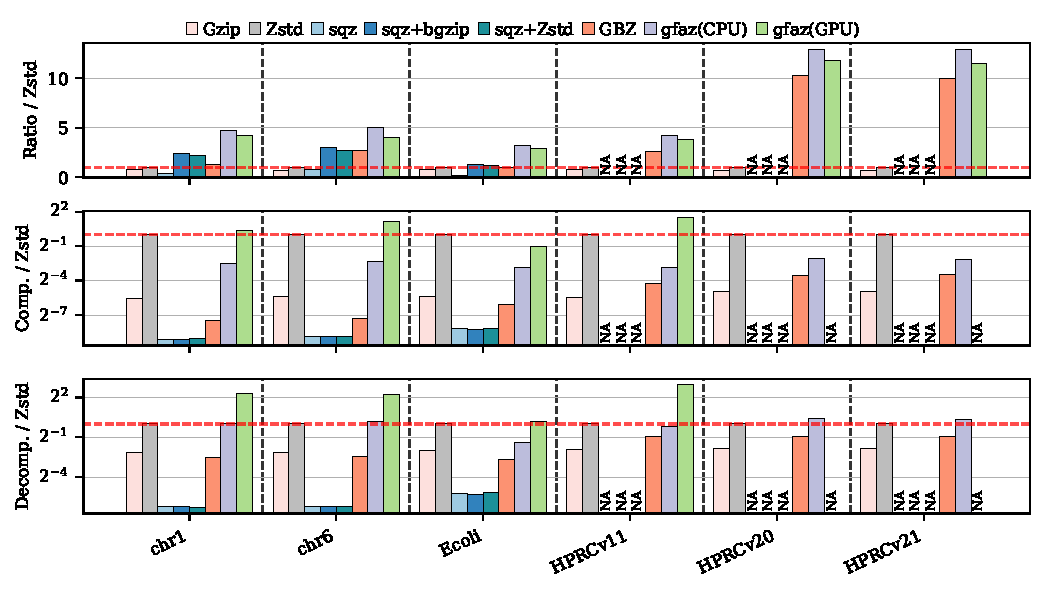
\includegraphics[width=\linewidth]{fig_eval_norm_combined.pdf}
  \caption{Normalized compression ratio, compression speed, and decompression speed relative to Zstd across all datasets. Results are normalized such that Zstd = 1.0 (dashed horizontal line). Speed metrics are plotted on a log scale (base 2).}
  \label{fig:eval-norm}
\end{figure*}


\begin{figure*}[t]
  \centering
  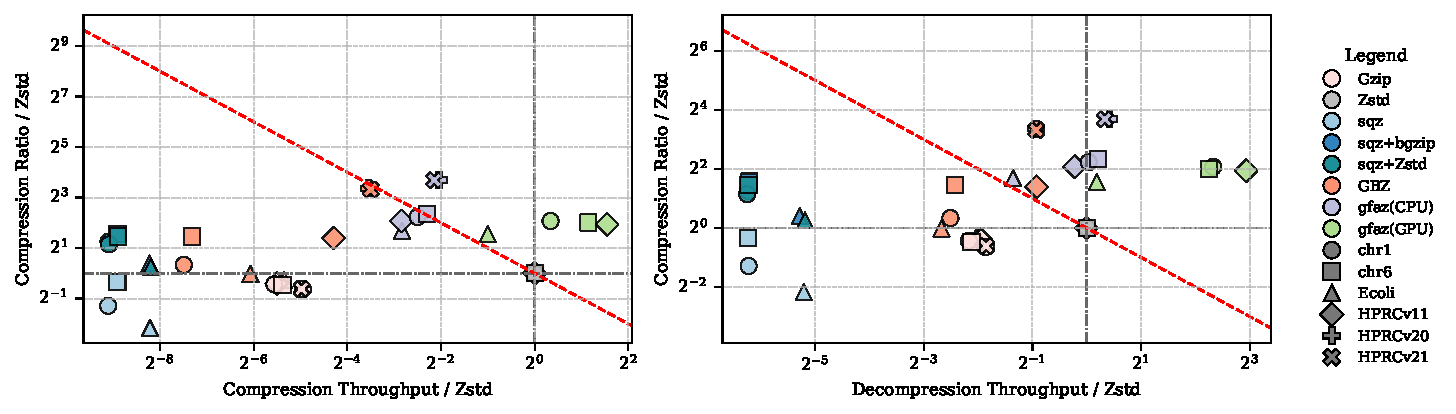
\includegraphics[width=\linewidth]{fig_pareto_combined.pdf}
  \caption{Pareto trade-off between compression ratio (y-axis) and speed (x-axis), normalized to Zstd (baseline at $1.0$). The dashed diagonal line ($y=1/x$) represents an iso-efficiency curve where a $2\times$ increase in ratio compensates for a $2\times$ drop in speed. Points above this line and to the right represent better trade-offs than the baseline.}
  \label{fig:pareto}
\end{figure*}


\begin{table*}[t]
  \centering
  \scriptsize
  \setlength{\tabcolsep}{3pt}
  \renewcommand{\arraystretch}{1.05}
  \caption{Ablation of \texttt{Compact} and \texttt{Sort} on rulebook effectiveness.
    Each cell shows \(H\) / \(L\), where \(H=r\gg32\) and \(L=r\,\&\,\texttt{0xffffffff}\); each entry is the ZSTD-compressed size followed by the compression ratio in parentheses.}
  \label{tab:compact-sort-ablation}
  \resizebox{\textwidth}{!}{%
    \setlength{\tabcolsep}{2pt}
\begin{tabular}{l|c|c|c|c}
  \hline
  \textbf{Dataset}    & \textbf{compact+sort} & \textbf{compact} & \textbf{sort} & \textbf{none} \\
  \hline
  EcoliGraph\_MGC     &
  53.9\,KB (\textbf{9.6$\times$}) / 215\,KB (\textbf{2.4$\times$})    &
  348\,KB (1.5$\times$) / 358\,KB (1.4$\times$)                       &
  70.7\,KB (9.6$\times$) / 291\,KB (2.3$\times$)                      &
  463\,KB (1.5$\times$) / 477\,KB (1.4$\times$)                       \\
  chr1.pan.smooth     &
  4.3\,MB (\textbf{11.2$\times$}) / 30.4\,MB (\textbf{1.6$\times$})   &
  40.6\,MB (1.2$\times$) / 40.6\,MB (1.2$\times$)                     &
  5.2\,MB (11.1$\times$) / 38.0\,MB (1.5$\times$)                     &
  50.0\,MB (1.2$\times$) / 50.0\,MB (1.2$\times$)                     \\
  chr6.pan.smooth     &
  2.0\,MB (\textbf{12.1$\times$}) / 14.0\,MB (\textbf{1.7$\times$})   &
  19.3\,MB (1.2$\times$) / 19.3\,MB (1.2$\times$)                     &
  2.4\,MB (12.0$\times$) / 17.8\,MB (1.6$\times$)                     &
  24.1\,MB (1.2$\times$) / 24.1\,MB (1.2$\times$)                     \\
  hprc-v1.1           &
  61.2\,MB (\textbf{10.2$\times$}) / 330\,MB (\textbf{1.9$\times$})   &
  565\,MB (1.1$\times$) / 561\,MB (1.1$\times$)                       &
  73.9\,MB (10.4$\times$) / 418\,MB (1.8$\times$)                     &
  697\,MB (1.1$\times$) / 692\,MB (1.1$\times$)                       \\
  hprc-v2.0           &
  124\,MB (\textbf{13.1$\times$}) / 1254\,MB (\textbf{1.3$\times$})   &
  1512\,MB (1.1$\times$) / 1513\,MB (1.1$\times$)                     &
  153\,MB (13.0$\times$) / 1558\,MB (1.3$\times$)                     &
  1857\,MB (1.1$\times$) / 1859\,MB (1.1$\times$)                     \\
  hprc-v2.1           &
  130\,MB (\textbf{13.1$\times$}) / 1315\,MB (\textbf{1.3$\times$})   &
  1588\,MB (1.1$\times$) / 1589\,MB (1.1$\times$)                     &
  161\,MB (12.9$\times$) / 1632\,MB (1.3$\times$)                     &
  1949\,MB (1.1$\times$) / 1951\,MB (1.1$\times$)                     \\
  \hline
\end{tabular}

  }
\end{table*}



\subsection{Compression-Decompression Performance}\label{subsec:compression-performance}

We include gzip and zstd as general-purpose baselines, GBZ and SQZ as pangenome-oriented compressors; for SQZ we also report \texttt{sqz+bgzip} and \texttt{sqz+zstd} to probe its best ratio under alternative back-end compressors.
SQZ runs out of memory on HPRC v1.1 and larger graphs, so those entries are marked NA.
SQZ and GBZ also drop parts of the original GFA representation, making the \gfaz comparisons conservative.
For the 300+\,GB HPRC v2.0/v2.1 graphs, the current GPU implementation runs out of device memory; we therefore report GPU ratios via a CPU simulation of the GPU rule-mining/encoding logic and omit GPU throughput for those two datasets.
Table~\ref{tab:ratio-throughput} reveals three consistent patterns.


\noindent \textbf{Insight 1 (ratio gains increase with graph complexity).}
\gfaz gives the best ratio on all datasets with available results, for both backends. On chr1, \gfaz(CPU) reaches 35.4$\times$ versus zstd 7.54$\times$ and GBZ 9.52$\times$; on chr6, 35.4$\times$ versus 6.99$\times$ and 19.2$\times$.
On larger HPRC graphs, the gap widens: on v2.0, \gfaz(CPU) reaches 83.9$\times$ versus zstd 6.49$\times$ and GBZ 66.8$\times$; on v2.1, 82.8$\times$ versus 6.43$\times$ and 64.2$\times$.
The GPU ratio is consistently but modestly below CPU (e.g., 31.7$\times$ vs 35.4$\times$ on chr1, 20.4$\times$ vs 22.4$\times$ on v1.1), consistent with checkerboard encoding (Section~\ref{subsec:gpu}) replacing fewer overlapping opportunities than serial greedy encoding in each round.
The ratio advantage is not specific to the HPRC pipeline. Table~\ref{tab:ratio-other} adds two graphs from other sources: HGSVC3, an $80.1$\,GB whole-genome Minigraph--Cactus pangenome from a different consortium, and a chromosome from the 1000-genome-scale 1KCP collection whose variation is carried entirely in graph topology (a reference-only GFA with no embedded haplotype paths). On both, \gfaz(CPU) again gives by far the best ratio---$28.1\times$ on HGSVC3 and $18.4\times$ on 1KCP-chr1, versus $4.0$--$4.5\times$ for gzip and $6.9$--$7.1\times$ for zstd.

\begin{table}[t]
\centering
\caption{Compression ratio on two graphs from outside the HPRC (single-run, ratio only). \gfaz retains its ratio advantage on a different-consortium pangenome (HGSVC3) and on a topology-only graph (1KCP-chr1).}
\label{tab:ratio-other}
\small
\begin{tabular}{lrrrr}
\hline
Dataset & GFA & Gzip & Zstd & \gfaz(CPU) \\
\hline
HGSVC3      & 80.1\,GB & 4.0$\times$ & 7.1$\times$ & \textbf{28.1$\times$} \\
1KCP-chr1   & 1.66\,GB & 4.5$\times$ & 6.9$\times$ & \textbf{18.4$\times$} \\
\hline
\end{tabular}
\end{table}

\noindent \textbf{Insight 2 (Throughput remains strong across CPU/GPU).}
When inputs fit GPU memory, \gfaz(GPU) is the fastest high-ratio operating point: on HPRC v1.1, it reaches 4843/9435 MB/s compression/decompression, versus \gfaz(CPU) at 231/1058 MB/s and zstd at 1657/1234 MB/s.
On chr1 and chr6, \gfaz(GPU) also leads throughput, showing that the GPU backend is most effective when traversal data can remain device-resident.
For v2.0/v2.1, GPU throughput is unavailable because the traversal stream exceeds device memory, but \gfaz(CPU) still gives the fastest decompression (1652 and 1559 MB/s) while retaining much higher ratios than zstd.
CPU compression is slower than zstd on these largest graphs, but this trade-off is favorable for storage and repeated-read workloads.
On the small \emph{E. coli} input, zstd compresses fastest, while \gfaz(GPU) still improves both ratio and decompression speed.

\noindent \textbf{Insight 3 (alternative methods occupy weaker ratio--speed fronts).}
SQZ variants can improve ratio over gzip/zstd on chromosome graphs, but their throughput (about 3--5 MB/s compression and about 20--35 MB/s decompression) is two orders of magnitude lower than \gfaz.
GBZ is the strongest non-\gfaz ratio baseline on large HPRC graphs, but remains below \gfaz in ratio (66.8$\times$/64.2$\times$ vs 83.9$\times$/82.8$\times$ on v2.0/v2.1) and decompression speed (648/652 vs 1652/1559 MB/s on CPU), while preserving fewer GFA semantics.

\begin{table}[t]
  \centering
  \scriptsize
  \setlength{\tabcolsep}{3pt}
  \renewcommand{\arraystretch}{1.05}
  \caption{Random-access evaluation using \texttt{extract-traversal}. We measure the time and peak memory required to reconstruct only 1, 4, or 16 selected paths/walks from an existing \texttt{.gfaz} file.}
  \label{tab:random-access}
  \resizebox{\columnwidth}{!}{%
    \begin{tabular}{lrrrr}
      \hline
      \textbf{Dataset} & \textbf{Extracted} & \textbf{Elapsed (s)} & \textbf{Peak Mem. (GB)} & \textbf{GFA Size (GB)} \\
      \hline
      \multirow{3}{*}{chr1}       & 1  & 0.102 & 0.38 & 7.1 \\
                                   & 4  & 0.103 & 0.37 & 7.1 \\
                                   & 16 & 0.106 & 0.41 & 7.1 \\
      \hline
      \multirow{3}{*}{hprc-v1.1}  & 1  & 1.006 & 4.09 & 48 \\
                                   & 4  & 1.012 & 4.10 & 48 \\
                                   & 16 & 1.029 & 4.13 & 48 \\
      \hline
      \multirow{3}{*}{hprc-v2.0}  & 1  & 2.285 & 9.26 & 358 \\
                                   & 4  & 2.302 & 9.28 & 358 \\
                                   & 16 & 2.312 & 9.30 & 358 \\
      \hline
      \multirow{3}{*}{hprc-v2.1}  & 1  & 2.278 & 9.65 & 369 \\
                                   & 4  & 2.303 & 9.67 & 369 \\
                                   & 16 & 2.380 & 9.74 & 369 \\
      \hline
    \end{tabular}
  }
\end{table}

\begin{table}[t]
  \centering
  \scriptsize
  \setlength{\tabcolsep}{5pt}
  \renewcommand{\arraystretch}{1.05}
  \caption{Incremental haplotype extension using \texttt{add-haplotypes}. Each run appends 50 new paths/walks using the rulebook already stored in the input \texttt{.gfaz} file.}
  \label{tab:incremental-extension}
  \resizebox{\columnwidth}{!}{%
    \begin{tabular}{lrrrr}
      \hline
      \textbf{Dataset} & \textbf{Added Haplotypes} & \textbf{Elapsed (s)} & \textbf{Peak Memory (GB)} & \textbf{GFA Size (GB)} \\
      \hline
      chr1       & 50 & 0.95  & 0.97  & 7.1 \\
      chr6       & 50 & 0.54  & 0.51  & 3.8 \\
      hprc-v1.1  & 50 & 3.25  & 3.25  & 48 \\
      hprc-v2.0  & 50 & 9.80  & 16.85 & 358 \\
      hprc-v2.1  & 50 & 10.20 & 17.32 & 369 \\
      \hline
    \end{tabular}
  }
\end{table}




\noindent \textbf{Normalized and Pareto views.}
Figures~\ref{fig:eval-norm} and~\ref{fig:pareto} summarize the same results normalized to Zstd. \gfaz consistently improves decompression and ratio efficiency.
For compression, only the small input can fall below the line but still keeps a substantial multi-fold ratio advantage over Zstd.



\subsection{Random Access and Incremental Extension}\label{subsec:random-access-eval}

We next evaluate the two traversal-centric operations enabled by the \texttt{.gfaz} layout: extracting a small number of haplotypes without full decompression, and appending new haplotypes without recompressing the entire file.

\noindent \textbf{Random access.}
Table~\ref{tab:random-access} reports extraction of 1, 4, or 16 paths/walks from existing \texttt{.gfaz} files. Runtime stays nearly flat as more records are requested. On HPRC v2.1 (369\,GB), extracting 1, 4, and 16 haplotypes takes 2.28\,s, 2.30\,s, and 2.38\,s, respectively. Peak memory also changes only slightly, from 9.65\,GB to 9.74\,GB.

\noindent \textbf{Incremental extension.}
Table~\ref{tab:incremental-extension} reports the cost of appending 50 new haplotypes. This takes 0.54--0.95\,s on chromosome-scale graphs, 3.25\,s on HPRC v1.1, and about 10\,s on the 358--369\,GB graphs. On HPRC v2.1, appending 50 haplotypes takes 10.2\,s, compared with roughly 1100\,s for full recompression.



\subsection{Ablation: Compact and Sort}\label{subsec:ablation-compact-sort}
We evaluate four workflow variants: \texttt{compact+sort} (full design), \texttt{compact} only, \texttt{sort} only, and \texttt{none}.
For each packed 64-bit rule ID \(r\), we split it into two 32-bit integer streams:
\(H = r \gg 32\) (high 32 bits) and \(L = r \,\&\, \texttt{0xffffffff}\) (low 32 bits) during compression, then entropy-code each stream with ZSTD.
Results directly validate the design rationale in Section~\ref{subsec:pipeline}.
Sorting is the dominant factor for \(H\): on chr1, \(H\) improves from 1.2$\times$ (\texttt{none}) to 11.1$\times$ (\texttt{sort}), and to 11.2$\times$ with \texttt{compact+sort}; similarly on hprc-v2.1, 1.1$\times$ (\texttt{none}) to 12.9$\times$ (\texttt{sort}) and 13.1$\times$ (\texttt{compact+sort}).
Compact then provides additional gains by removing unused rules and shrinking emitted streams: for chr1 \(L\) improves from 1.5$\times$ (\texttt{sort}) to 1.6$\times$ (\texttt{compact+sort}), and for hprc-v2.1 from 1.3$\times$ to 1.3$\times$ with a concrete size drop (1632\,MB to 1315\,MB).
Compared with \texttt{compact} only, the full \texttt{compact+sort} pipeline is consistently much better on \(H\) (e.g., chr6: 12.1$\times$ vs 1.2$\times$), showing that compacting without ordering does not create enough entropy structure for the rulebook.
This also clarifies a weakness of SQZ: although SQZ is grammar-based, highly variable rule symbols without strong ordering reduce rule-stream regularity, making entropy coding less effective than the sorted rulebook layout used by \gfaz.


\begin{table}[t]
  \centering
  \scriptsize
  \setlength{\tabcolsep}{4pt}
  \renewcommand{\arraystretch}{1.05}
  \caption{CPU stage-level profiling for compression and decompression.
    Share is computed as \texttt{time / stage total}.}
  \label{tab:cpu-breakdown}
  \resizebox{\columnwidth}{!}{%
    \setlength{\tabcolsep}{2pt}
\begin{tabular}{l r r r}
  \hline
  \textbf{Stage}                     & \textbf{Time (ms)} & \textbf{Tput (GB/s)} & \textbf{Share} \\
  \hline
  \multicolumn{4}{l}{\textit{Compression (total: 19888.78\,ms)}}                                  \\
  Grammar subtotal                   & 11004.68            & 0.20                  & 55.3\%         \\
  \quad generate\_rules              & 6000.89             & 0.38                  & 30.2\%         \\
  \quad encode\_traversals           & 4785.13             & 0.47                  & 24.1\%         \\
  \quad compact\_sort\_remap         & 196.83              & 11.5                  & 1.0\%          \\
  \quad split+delta\_encode          & 27.93               & 3.30                  & 0.1\%          \\
  \quad zstd compress                & 467.58              & 0.47                  & 2.4\%          \\
  Others                             & 8884.10             & --                    & 44.7\%         \\
  \hline
  \multicolumn{4}{l}{\textit{Decompression (total: 4221.47\,ms)}}                                 \\
  Grammar subtotal                   & 511.52              & 4.32                  & 12.1\%         \\
  \quad zstd decompress              & 102.39              & 1.60                  & 2.4\%          \\
  \quad decode rules (prefix sum)    & 2.85                & 32.4                  & 0.1\%          \\
  \quad expand traversals            & 371.93              & 6.06                  & 8.8\%          \\
  \quad decode traversals (pfx sum)  & 34.35               & 65.6                  & 0.8\%          \\
  Others                             & 3709.95             & --                    & 87.9\%         \\
  \hline
\end{tabular}

  }
\end{table}

\begin{table}[t]
  \centering
  \scriptsize
  \setlength{\tabcolsep}{4pt}
  \renewcommand{\arraystretch}{1.05}
  \caption{GPU stage-level profiling for compression and decompression.
    Share is computed as \texttt{time / stage total}.}
  \label{tab:gpu-breakdown}
  \resizebox{\columnwidth}{!}{%
    \setlength{\tabcolsep}{2pt}
\begin{tabular}{l r r r}
  \hline
  \textbf{Stage}                     & \textbf{Time (ms)} & \textbf{Tput (GB/s)} & \textbf{Share} \\
  \hline
  \multicolumn{4}{l}{\textit{Compression (total: 2322.85\,ms)}}                                   \\
  Grammar subtotal                   & 571.85              & 3.96                  & 24.6\%         \\
  \quad find\_max\_abs               & 5.96                & 378.0                 & 0.3\%          \\
  \quad delta\_encode                & 5.64                & 400.0                 & 0.2\%          \\
  \quad find\_repeated\_2mers        & 195.59              & 11.5                  & 8.4\%          \\
  \quad create\_rule\_table          & 18.36               & 122.8                 & 0.8\%          \\
  \quad apply\_2mer\_rules           & 105.24              & 21.4                  & 4.5\%          \\
  \quad compact\_rules\_remap        & 25.68               & 87.8                  & 1.1\%          \\
  \quad sort\_rules\_remap           & 16.70               & 135.0                 & 0.7\%          \\
  \quad split+delta\_encode          & 0.90                & 102.2                 & 0.0\%          \\
  \quad Zstd compress (nvComp)       & 197.78              & 11.4                  & 8.5\%          \\
  Others                             & 1751.00             & --                    & 75.4\%         \\
  \hline
  \multicolumn{4}{l}{\textit{Decompression (total: 876.00\,ms)}}                                  \\
  Grammar subtotal                   & 117.00              & 19.3                  & 13.4\%         \\
  \quad Zstd decompress (nvComp)     & 85.85               & 26.3                  & 9.8\%          \\
  \quad decode rules (prefix sum)    & 0.44                & 367.2                 & 0.1\%          \\
  \quad expand traversals            & 24.73               & 91.2                  & 2.8\%          \\
  \quad decode traversals (pfx sum)  & 5.98                & 377.1                 & 0.7\%          \\
  Others                             & 759.00              & --                    & 86.6\%         \\
  \hline
\end{tabular}

  }
\end{table}



\begin{table}[t]
  \centering
  \scriptsize
  \setlength{\tabcolsep}{3pt}
  \renewcommand{\arraystretch}{1.05}
  \caption{CPU peak resident memory using 16 threads for compression, a legacy decompression baseline that fully materializes the in-memory \texttt{GfaGraph}, and the implemented streaming decompression path.}
  \label{tab:cpu-memory}
  \resizebox{\columnwidth}{!}{%
    \begin{tabular}{lrrrr}
      \hline
      \textbf{Dataset} & \textbf{Comp.} & \textbf{Full-Graph} & \textbf{Streaming} & \textbf{GFA} \\
      \textbf{} & \textbf{Peak (GB)} & \textbf{Decomp. (GB)} & \textbf{Decomp. (GB)} & \textbf{Size (GB)} \\
      \hline
      chr1       & 7.4   & 6.3   & 0.98 & 7.1 \\
      chr6       & 3.2   & 3.0   & 0.66 & 3.8 \\
      Ecoli      & 0.24  & 0.18  & 0.18 & 0.113 \\
      hprc-v1.1  & 45    & 37    & 3.4  & 48 \\
      hprc-v2.0  & 343   & 289   & 19.3 & 358 \\
      hprc-v2.1  & 356   & 295   & 20.7 & 369 \\
      \hline
    \end{tabular}
  }
\end{table}



\subsection{Performance Breakdown}\label{subsec:breakdown}
Tables~\ref{tab:gpu-breakdown} and~\ref{tab:cpu-breakdown} break down stage-level profiling for the GPU and CPU backends respectively. Each table reports a \texttt{Grammar subtotal} (traversal-related stages) and \texttt{Others} (all remaining fields---segment sequences, link/jump/containment columns, optional fields, and their associated ZSTD encoding).

On both backends, decompression is dominated by \texttt{Others}: 87.9\% on CPU and 86.6\% on GPU, leaving only 12.1\% (CPU) and 13.4\% (GPU) in grammar stages.
Within grammar decode, traversal expansion itself is fast (371.93\,ms at 6.06\,GB/s on CPU; 24.73\,ms at 91.2\,GB/s on GPU), consistent with one-pass expansion and \(O(1)\) rule lookup (\texttt{rule\_id - min\_rule\_id}).
This supports the design claim that traversal reconstruction is not the end-to-end bottleneck once the rulebook is available.

The two backends differ mainly in compression cost distribution.
On CPU, grammar stages consume 55.3\% of compression time, with \texttt{generate\_rules} (30.2\%) and \texttt{encode\_traversals} (24.1\%) as dominant kernels.
On GPU, grammar drops to 24.6\% of total compression time (\texttt{find\_repeated\_2mers} 8.4\%, \texttt{apply\_2mer\_rules} 4.5\%), while \texttt{Others} rises to 75.4\%, consistent with nvComp/ZSTD orchestration overhead in the current pipeline.
This profile explains why the GPU grammar algorithm is already fast but end-to-end speedups are now limited by entropy and non-traversal stages.

\subsection{CPU Memory Profiling}\label{subsec:cpu-memory}

Table~\ref{tab:cpu-memory} compares three CPU memory profiles measured with 16 threads: compression, a legacy decompression baseline that fully materializes the entire \texttt{GfaGraph}, and the implemented streaming decompression path that expands one path/walk and writes it out immediately. The fully materialized baseline reaches 37\,GB, 289\,GB, and 295\,GB on HPRC v1.1, v2.0, and v2.1, respectively. In contrast, the implemented streaming path reduces peak decompression memory to 3.4\,GB, 19.3\,GB, and 20.7\,GB, a reduction of about \(14\text{--}15\times\).

High compression peak memory is less critical in practice for three reasons. First, it occurs primarily in the first rule-encoding round and drops quickly afterward as the traversal stream shrinks. Second, compression is usually a one-time preprocessing step, whereas decompression and downstream analyses are run repeatedly. Third, downstream graph tools such as VG~\cite{garrison2018variation} and ODGI~\cite{guarracino2022odgi} already require memory footprints larger than the input GFA size.


\section{\gfaz as a Compute Engine}\label{sec:compute}

The previous sections present \gfaz as a compressor. The same representation also
supports a broader systems role: \gfaz can act as a compute substrate for
path-centric pangenome analyses. Many downstream tasks do not require arbitrary
mutation of the graph. Instead, they repeatedly scan haplotype traversals and
fold node visits into a compact accumulator: a coverage histogram, a
window-by-sample matrix, or an allele table relative to a reference path. Because
\texttt{.gfaz} already stores P/W traversals as grammar-compressed integer
streams, these analyses can consume the compressed traversal store directly and
avoid reconstructing the full GFA text or a whole-graph object.

This section describes the compute-engine design. The central abstraction is a
streaming traversal primitive that expands grammar rules on demand and emits
orientation-signed node IDs to an analysis-specific visitor
(Section~\ref{subsec:ce-model}). A bounded rule-leaf cache exposes a
memory/recompute trade-off for workloads that repeatedly touch large rules
(Section~\ref{subsec:ce-cache}). The resulting memory footprint is the compressed
traversal store plus the workload accumulator, rather than the decompressed
traversal graph (Section~\ref{subsec:ce-memory}). We instantiate the model in
three commands---\texttt{growth}, \texttt{pav}, and \texttt{deconstruct}---that
share the same decode substrate but use different accumulators
(Section~\ref{subsec:ce-instances}).

\subsection{Motivation: Avoiding Materialization}\label{subsec:ce-motivation}

Pangenome analysis tools often begin by materializing a representation larger
than the statistic they ultimately compute. Panacus~\cite{parmigiani2024panacus}
parses GFA path and walk records into item tables before deriving growth and core
curves. odgi~\cite{guarracino2022odgi} builds a succinct whole-graph object
before running operations such as \texttt{odgi pav}. \texttt{vg deconstruct}
loads a graph and snarl decomposition before emitting a reference-relative VCF
from traversals~\cite{garrison2018variation,hickey2020genotyping}. These
representations are appropriate for general graph operations, but for
path-centric folds the resident object can dominate both memory and time.

\gfaz targets a narrower but common execution pattern: compressed traversal
stream $\rightarrow$ small accumulator $\rightarrow$ biological statistic. The
design deliberately does not try to replace topology-heavy graph libraries.
Instead, it exploits the fact that the dominant GFA component---haplotype
traversals---is already encoded in a streamable form. The analysis pays only for
the compressed traversal columns, the rulebook needed to expand them, and the
state required by the specific query.

\subsection{Execution Model: Streaming Leaf Expansion}\label{subsec:ce-model}

\paragraph{Compressed traversal store.}
The \texttt{.gfaz} container stores P traversals and W traversals as two flat
\texttt{int32} arrays. Each record has an encoded-length column, and the original
pre-compression traversal lengths are retained for workflows that need a
materialized fallback. ZSTD decompression of these blocks yields
grammar-compressed integer streams containing literals and rule IDs, but not the
fully expanded node sequences. The engine slices the flat arrays into zero-copy
\texttt{HapSlice} views:
\[
  \{\texttt{pointer},\ \texttt{encoded length},\ \texttt{original length}\}.
\]
The grammar rulebook is stored as two parallel \texttt{int32} arrays,
\texttt{rules\_first} and \texttt{rules\_second}, delta-decoded once after ZSTD
decompression. The first rule ID, \texttt{min\_rule\_id}, is read from the layer
metadata; \texttt{max\_rule\_id} is derived from the rule count. A value whose
absolute ID lies in this half-open range is a rule, and all other values are
literals. This single-comparison classification is sound because compression
reserves the rule namespace strictly above every literal node ID
(Section~\ref{subsec:pipeline}): rule IDs are assigned sequentially across rounds
starting from \texttt{start\_id}, so a decoder never has to consult a side table
to tell a node from a rule.

\paragraph{Streaming primitive.}
The reusable operation is:
\[
  \textsc{StreamDecodedNodes}(\texttt{HapSlice},\ \textsc{Visit}).
\]
It emits the decoded orientation-signed node IDs of one traversal, in order, to a
caller-supplied visitor. For each encoded element $e$, the decoder performs one
boundary check. If $|e|$ is outside the rule range, $e$ is a literal. Otherwise
the decoder indexes the rule arrays at $|e|-\texttt{min\_rule\_id}$ and expands
the two children recursively. A negative rule reference denotes the
reverse-complement orientation: the children are visited in reverse order and
their signs are flipped. Thus the same rulebook serves both strands without
duplicating rules.

The inverse-delta transform is fused into streaming. For the common
\texttt{delta\_round=1} case, the decoder keeps a running prefix sum and calls
the visitor immediately after reconstructing each node ID. For
\texttt{delta\_round=0}, literals and rule leaves are already in node-ID space.
For uncommon higher delta counts, the implementation materializes one traversal,
applies the required inverse passes, and then visits the recovered nodes.

\begin{algorithm}[t]
  \caption{Streaming traversal expansion for \texttt{delta\_round} 0 or 1}
  \label{alg:ce-stream}
  \begin{algorithmic}[1]
    \REQUIRE slice $E$, rule range $[m,M)$, rule arrays $R_1,R_2$,
             delta round $D \in \{0,1\}$, visitor \textsc{Visit}
    \STATE $\textit{prev} \gets 0$
    \STATE \textbf{define} \textsc{Emit}($v$):
    \IF{$D = 1$}
      \STATE $\textit{prev} \gets \textit{prev} + v$; \textsc{Visit}(\textit{prev})
    \ELSE
      \STATE \textsc{Visit}($v$)
    \ENDIF
    \STATE \textbf{define} \textsc{Expand}($r$, \textit{reverse}):
    \STATE \quad $(a,b) \gets (R_1[r-m], R_2[r-m])$
    \STATE \quad $(c_1,c_2) \gets \textit{reverse}\,?\,(b,a):(a,b)$
           \COMMENT{reverse swaps child order}
    \FORALL{$c \in (c_1,c_2)$}
      \IF{$|c| \in [m,M)$}
        \STATE \textsc{Expand}($|c|$, $\,\textit{reverse}\oplus(c<0)$)
               \COMMENT{rule child: fold parent and child orientation}
      \ELSE
        \STATE \textsc{Emit}($\textit{reverse}\,?\,{-}c:c$)
               \COMMENT{literal child: flip sign under reverse}
      \ENDIF
    \ENDFOR
    \FORALL{$e \in E$ in order}
      \IF{$|e| \in [m,M)$}
        \STATE \textsc{Expand}($|e|$, $e < 0$)
      \ELSE
        \STATE \textsc{Emit}($e$)
      \ENDIF
    \ENDFOR
  \end{algorithmic}
\end{algorithm}

The cost of decoding one traversal is linear in the expanded traversal length.
Rule resolution is an array lookup, not a hash lookup, and recursion depth is
bounded by the number of grammar rounds. The visitor is templated in the
implementation, so the per-node fold can be inlined through the decode loop.

\subsection{Rule-Leaf Cache}\label{subsec:ce-cache}

On-demand recursion avoids materializing all expanded traversals, but a large
rule may be referenced many times. For workloads where repeated rule expansion is
noticeable, \gfaz provides a bounded \texttt{RuleLeafCache}. The cache stores the
fully expanded forward leaf sequence for any rule whose expansion fits within a
user-specified byte budget. Reverse expansion is derived by scanning the cached
leaf sequence backward and negating signs, so no reverse copy is stored.

Cache construction is bottom-up over rule IDs. A rule is admitted only if its
children have already been expanded or can be represented lazily and if the
projected leaf sequence fits within the remaining budget. Rules that do not fit
fall back to recursive expansion, preserving correctness for every budget. The
cache is built once, then shared read-only by all decoding threads. A budget of
zero recovers fully lazy expansion; larger budgets trade memory for less repeated
recursion. In the current implementation, \texttt{pav} and \texttt{deconstruct}
enable this cache, while \texttt{growth} uses pure recursive expansion.

\subsection{Memory Model}\label{subsec:ce-memory}

The compute engine replaces decompressed traversal materialization with four
resident components:
\begin{enumerate}[noitemsep, topsep=2pt, leftmargin=*]
  \item \textbf{Grammar-compressed traversal store}: ZSTD-decompressed but still
        grammar-encoded P/W integer streams, encoded-length columns, and the
        rule arrays.
  \item \textbf{Optional rule-leaf cache}: bounded by a configurable byte
        budget.
  \item \textbf{Analysis accumulator}: the state required by the specific query,
        such as a node coverage vector, a CSR node-to-group index, or a per-site
        allele table.
  \item \textbf{Sequence payload when needed}: \texttt{deconstruct} additionally
        keeps segment DNA resident so it can spell REF and ALT alleles.
\end{enumerate}

The key distinction is that the traversal store remains grammar-compressed.
Memory still scales with the size of the compressed traversal columns and with
the query accumulator, but not with a fully expanded list of all path and walk
steps. This property is most useful for workloads that scan many haplotypes but
retain only aggregate state.

\subsection{Parallelization}\label{subsec:ce-parallel}

Traversal decoding is parallel over \texttt{HapSlice} objects. The flat traversal
arrays, rulebook, segment sequence payload, and rule-leaf cache are read-only
after setup, so distinct threads can decode distinct traversals without
synchronizing on the decode path. Because expanded traversal lengths vary widely
across haplotypes, the parallel loops use dynamic OpenMP scheduling for load
balance. Synchronization is pushed into the workload-specific fold, and the three
commands cover distinct accumulator policies:
\begin{itemize}[noitemsep, topsep=2pt, leftmargin=*]
  \item \textbf{\texttt{growth}} parallelizes over haplotype groups and shares a
        single node coverage array. Each thread keeps a private last-seen stamp
        array to suppress duplicate counts within a group, and performs an atomic
        increment only on the first visit of a node in that group; the stamp is a
        rolling byte that is reset when it wraps, avoiding a per-group clear of
        the stamp array. The coverage-to-histogram reduction is then computed with
        per-thread local histograms merged in a short critical section, and the
        closed-form growth curve is evaluated in parallel over cohort sizes.
  \item \textbf{\texttt{pav}} decodes each traversal into a private sorted-unique
        node set (lock-free, per-slice slots), reference slices additionally
        capturing their ordered node stream. A serial prefix-sum builds the CSR
        node-to-group index, after which the per-contig reference sweep runs in
        parallel and updates the output matrix with atomics; these are
        contention-free in the common case because distinct contigs map to
        disjoint window-index ranges.
  \item \textbf{\texttt{deconstruct}} first fixes sites with a single
        linear-time topology pass (the biconnected decomposition below), which
        decodes no haplotype, then streams haplotypes in parallel into per-thread
        observation buffers concatenated after the parallel region; site assembly
        and VCF formatting are a subsequent serial pass over the per-site
        observation groups.
\end{itemize}

This organization separates the shared decoding substrate from the accumulator
policy, and isolates each command's serial stages (the CSR build for \texttt{pav},
site assembly for \texttt{deconstruct}). It also leaves a clear GPU path:
per-slice rule expansion is regular integer work over contiguous arrays, while the
fold can be specialized for each analysis.

\subsection{Three Instantiations}\label{subsec:ce-instances}

All three implemented commands share the same setup. They deserialize
\texttt{CompressedData}, ZSTD-decompress the rulebook and P/W traversal blocks,
delta-decode the rule arrays, build \texttt{HapSlice} views, and reconstruct only
the metadata columns needed for grouping or reference lookup.


\noindent\textbf{Growth.}
This command computes Panacus-style union growth for nodes. P/W records are
grouped by one of several identities: per record, PanSN sample,
sample-haplotype, or sample-haplotype-sequence. For P-lines the identity is parsed
from the path name with a PanSN matcher (mirroring Panacus, including the
stripping of trailing \texttt{:start-end} coordinate suffixes); for W-lines the
sample, haplotype index, and sequence ID are already stored as separate columns
and need no parsing. Streaming one group updates a coverage array
$\texttt{cov}[v]$, where each node is counted at most once per group. The coverage
vector is reduced to a histogram $\texttt{hist}[c]=|\{v:\texttt{cov}[v]=c\}|$. For
a pangenome with $N$ groups, the expected number of nodes observed in a random
subset of size $k$ is
\[
  \texttt{growth}[k]
    =
  \sum_c \texttt{hist}[c]
    \left(1-\frac{\binom{N-c}{k}}{\binom{N}{k}}\right).
\]
The ratio $\binom{N-c}{k}/\binom{N}{k}$ is evaluated as the stable product
$\prod_{i=0}^{c-1}(N-k-i)/(N-i)$ rather than by forming the binomial coefficients,
which would overflow at pangenome $N$. The accumulator is linear in the number of
nodes, and this fold matches Panacus union-growth semantics (count $=$ node,
coverage $\ge 1$, quorum $\ge 0$).

\noindent\textbf{PAV.}
This command computes a window-by-group matrix over BED intervals on reference
paths or walks, in three passes over a shared read-only decode state. \emph{Pass~1}
decodes every traversal once into a private sorted-unique node set; reference
traversals (those a BED \texttt{chrom} resolves to) additionally retain their
ordered node stream, captured as a side effect of the same decode so no reference
is decoded twice. \emph{Pass~2} unions the per-slice node sets of each group and
flattens the result into a compressed-sparse-row $\text{node}\rightarrow\text{groups}$
index: a counting pass tallies the groups per node, an exclusive prefix sum forms
the row offsets, and a cursor scatter fills the group-ID column. CSR is chosen over
a $\text{node}\rightarrow\text{list}$ map to remove the per-node container header
overhead, which is significant when the node count reaches hundreds of millions.
The rule-leaf cache is released after Pass~1, since Passes~2--3 perform no further
grammar expansion. \emph{Pass~3} sweeps each reference stream, maintaining a
running genomic offset from the segment-length column so that each visited node
maps to a half-open base interval; the BED ranges for that contig, pre-sorted by
start, are intersected against the node interval with an advancing range cursor,
and the resulting $(\text{window},\text{node})$ pairs are deduplicated. For each
unique pair, the node length is added to the window denominator and to the
numerator of every group in that node's CSR row. Groups are formed by the same
identity modes as \texttt{growth} (per record, sample, or sample-haplotype). A
node counts at most once per group, matching \texttt{odgi pav} semantics; the
result is node-length-weighted PAV ratios computed without a whole-graph object.

\noindent\textbf{Deconstruct.}
The \texttt{deconstruct} command is the most topology-sensitive instance of the
compute engine. It derives a reference-relative VCF from the compressed traversal
store without materializing all haplotype paths or constructing a general-purpose
whole-graph index. Each reference contig is decoded once to an orientation-signed
node stream \texttt{ref\_nodes}; a prefix sum over segment lengths maps reference
node positions to genomic offsets and gives the contig length used in the VCF
header. Site discovery and allele observation are separated. The paper-relevant
\texttt{--vg-compat} mode defines sites from top-level snarls with a new global
BCC algorithm over the topology stored in the compressed container. Allele
observation remains the same path-centric fold as the other compute-engine
commands: each compressed haplotype is streamed once through compact
site-boundary state.

Existing deconstruction pipelines typically combine graph loading, snarl
decomposition, and path inspection inside a materialized graph representation. In
\gfaz, the BCC algorithm keeps site discovery off the haplotype hot path. It
builds an orientation-aware node-end graph from the stored L-line topology: each
segment $s$ contributes two vertices, $s.5'$ and $s.3'$, joined by a \emph{black}
edge, and each GFA link contributes one \emph{grey} edge between the source
departure end and target arrival end. This is the bidirected ``interval'' graph
used by snarl theory, where snarls in a bidirected genome graph correspond to
biconnected blocks in a doubled/node-end representation~\cite{paten2018superbubbles}.
The black segment edges are essential for inversions: a single-node inversion
closes through the segment's two ends and is recovered as one biconnected block,
whereas a collapsed segment graph can expose the inverted segment as an
articulation point and split the site.

\gfaz\ runs an iterative Hopcroft--Tarjan decomposition over this node-end graph
(Algorithm~\ref{alg:ce-bcc}). The traversal maintains discovery times, low-link
values, and an edge stack; when returning from child $w$ to parent $u$, the
condition $\textit{low}(w)\ge\textit{disc}(u)$ pops one maximal biconnected block.
The pass is iterative rather than recursive to avoid call-stack limits on
chromosome-scale graphs, and runs in $O(V+E)$ time with linear auxiliary space.
Each non-trivial block is projected onto \texttt{ref\_nodes}: if the first and
last reference positions touched by the block define a clean span whose positions
all belong to the block and contain no repeated segment, the span is emitted as a
candidate top-level snarl. This filter rejects cyclic or ambiguous reference
traversals, while nested child bubbles and chains of leaf bubbles collapse into
their enclosing top-level snarl, matching the default record granularity of
\texttt{vg deconstruct}.

\begin{algorithm}[t]
  \caption{Top-level snarl extraction via biconnected decomposition}
  \label{alg:ce-bcc}
  \begin{algorithmic}[1]
    \REQUIRE links $L$; reference node stream \texttt{ref}; segment count $n$
    \STATE build node-end graph $G$: vertices $\{s.5',s.3'\}$ per segment $s$;
           \emph{black} edge $(s.5',s.3')$; \emph{grey} edge
           $(\textsc{dep}(a),\textsc{arr}(b))$ per link $a{\to}b$
    \STATE $t \gets 0$;\quad edge stack $\Sigma \gets [\,]$;\quad
           $\textit{disc}[\cdot]\gets 0$
    \STATE \textbf{procedure} \textsc{Dfs}($u$, $\textit{pe}$): \COMMENT{entered via edge \textit{pe}}
    \STATE \quad $\textit{disc}[u]\gets\textit{low}[u]\gets (t\gets t{+}1)$
    \STATE \quad \textbf{for each} incident edge $e=(u,w)\neq \textit{pe}$:
    \STATE \qquad \textbf{if} $\textit{disc}[w]=0$: \quad push $e$ on $\Sigma$;\;
           \textsc{Dfs}($w$,$e$);\;
           $\textit{low}[u]\gets\min(\textit{low}[u],\textit{low}[w])$
    \STATE \qquad\quad \textbf{if} $\textit{low}[w]\ge\textit{disc}[u]$:
           pop $\Sigma$ down to and including $e$ as block $B$;\; \textsc{Project}($B$)
    \STATE \qquad \textbf{else if} $\textit{disc}[w]<\textit{disc}[u]$:
           push $e$ on $\Sigma$;\; $\textit{low}[u]\gets\min(\textit{low}[u],\textit{disc}[w])$
    \STATE \textbf{for each} reference segment $s$ and end $x\in\{s.5',s.3'\}$ with $\textit{disc}[x]=0$: \textsc{Dfs}($x$, \textsc{nil})
    \STATE \textbf{procedure} \textsc{Project}($B$):
    \STATE \quad $S \gets$ segments incident to $B$;\quad
           $I \gets \{\,i : \texttt{ref}[i]\in S\,\}$
    \STATE \quad \textbf{if} $|B|\ge 2$ \textbf{and} $|I|\ge 2$:
           $(\ell,h)\gets(\min I,\max I)$
    \STATE \qquad \textbf{if} \texttt{ref}$[\ell..h]$ repeats no segment \textbf{and}
           $\texttt{ref}[i]\in S\ \forall i\in[\ell,h]$:
           emit snarl $(\texttt{ref}[\ell],\texttt{ref}[h])$
    \STATE reduce emitted snarls to a non-overlapping chain by position
  \end{algorithmic}
\end{algorithm}

Once BCC sites are fixed, \gfaz\ returns to the compressed traversal substrate.
For every top-level snarl, it stores forward and reverse entrance maps. The
forward entrance maps the reference source boundary to the snarl and expects the
reference sink as its exit; the reverse entrance maps the reverse-complement sink
to the same snarl and expects the reverse-complement source, allowing inverted
haplotype traversals to be normalized back into the reference frame. During
streaming, a small state machine is either closed or associated with one open
snarl (Algorithm~\ref{alg:ce-snarl}). A boundary opens a site, ordinary decoded
nodes are appended to a small interior buffer, and the matching exit emits that
interior tagged by the haplotype slice. If traversal was reversed through the
site, the buffer is scanned backward and signs are negated before emission; a
boundary may close one site and immediately open the next, which handles adjacent
snarls without retaining the surrounding path.

\begin{algorithm}[t]
  \caption{Streaming allele observation for one haplotype (snarl mode)}
  \label{alg:ce-snarl}
  \begin{algorithmic}[1]
    \REQUIRE slice $E$; per-snarl boundary maps \textsc{Entrance} (node-side
    $\rightarrow$ snarl, forward or reversed) and exit node-sides
    \STATE $open \gets \bot$; $\textit{interior} \gets [\,]$
    \STATE \textbf{for each} decoded node $u$ of $E$ (Algorithm~\ref{alg:ce-stream}):
    \STATE \quad $v \gets$ node-side vertex of $u$
    \IF{$open = \bot$}
      \STATE \textsc{TryOpen}($v$): if $v$ is a (forward/reversed) entrance, set
      $open$, \textit{reversed}, $\textit{exit}$, $\textit{interior}\gets[\,]$
    \ELSIF{$v = \textit{exit}$}
      \STATE emit interior for snarl $open$ (reverse + negate if \textit{reversed}),
      tagged with this slice
      \STATE $open \gets \bot$; \textsc{TryOpen}($v$) \COMMENT{exit may open a chained snarl}
    \ELSE
      \STATE append $u$ to \textit{interior}
    \ENDIF
  \end{algorithmic}
\end{algorithm}

Per site, the reference interior spells allele $0$; each observed interior is
spelled by concatenating segment DNA (reverse-oriented nodes contributing reverse
complements) and deduplicated to an allele index. A site with no alternate allele
is dropped. Equal-length alleles are emitted as substitutions; otherwise the
record is left-anchored with the last base of the source anchor, following the
standard VCF indel convention. \texttt{INFO} carries \texttt{AC}/\texttt{AN}/
\texttt{AF} and the number of samples with data, and an optional
\texttt{--max-site-length} guard collapses very large spans to a symbolic
\texttt{<CPX>} record. Haplotypes collapse into VCF sample columns by the chosen
grouping mode, with one genotype slot per haplotype index so reference-tiling
contigs resolve to the sample's true ploidy rather than inflating it. Records are
emitted in sorted genomic order per contig, yielding a GFAz-native
reference-relative deconstruction workflow computed directly on compressed
traversals.

These three commands delimit the intended scope of the compute engine: analytics
whose hot path is traversal streaming plus a compact fold. Operations that require
arbitrary node-to-step queries, graph editing, or full topology transformation
remain better served by materialized graph toolkits.


\section{Evaluation Results}\label{sec:eval-results}

We evaluate the three headline analyses of Section~\ref{sec:compute}
against the standard tool for each task: \texttt{deconstruct} versus
\texttt{vg deconstruct}~\cite{garrison2018variation}, \texttt{growth} versus
Panacus~\cite{parmigiani2024panacus}, and \texttt{pav} versus
\texttt{odgi pav}~\cite{guarracino2022odgi}. All runs were performed on a single
node with an AMD Ryzen Threadripper PRO 9955WX (16 physical cores, 32 hardware
threads) and 503\,GiB of RAM. Each command was run at \textbf{1} and \textbf{16}
threads, one at a time, and wrapped in \texttt{/usr/bin/time\,-v} to record
wall-clock time and peak resident set size (RSS). \gfaz reads the compressed
\texttt{.gfaz} container directly; the baselines read the uncompressed GFA
(\texttt{odgi} additionally builds an \texttt{.og} index first, timed
separately).

\begin{table}[t]
\centering
\caption{Evaluation graphs. \gfaz operates on the compressed container, which is
$18$--$35\times$ smaller than the GFA the baselines must read.}
\label{tab:eval-datasets}
\small
\begin{tabular}{lrrr}
\hline
Graph & GFA & \texttt{.gfaz} & Ratio \\
\hline
chr1 (HPRC, smoothed) & 7.58\,GB & 214\,MB & 35.4$\times$ \\
chr6 (HPRC, smoothed) & 4.06\,GB & 115\,MB & 35.4$\times$ \\
\emph{E. coli} (MGC)  & 118\,MB  & 6.4\,MB & 18.4$\times$ \\
\hline
\end{tabular}
\end{table}

The chr1 and chr6 graphs are human pangenome graphs with a linear CHM13
reference, used for \texttt{deconstruct} and \texttt{pav}; the \emph{E. coli}
graph is a 13-strain bacterial pangenome used for \texttt{growth}. (The bacterial
graph is circular and stores only W-line walks, so it is not a meaningful target
for reference-anchored \texttt{deconstruct} nor for \texttt{odgi pav}, which does
not load W-line paths; it is retained as a \texttt{growth} data point.)

\subsection{Deconstruct (GFA\,$\rightarrow$\,VCF)}\label{subsec:eval-deconstruct}

Table~\ref{tab:eval-deconstruct} reports the GFA\,$\rightarrow$\,VCF
deconstruction of the chr1 and chr6 graphs against \texttt{vg deconstruct}.
\gfaz produces the same set of variant sites as \texttt{vg}---the record counts
agree to within $0.13\%$ (chr1: $1{,}593{,}901$ vs.\ $1{,}593{,}958$; chr6:
$1{,}304{,}123$ vs.\ $1{,}302{,}387$), consistent with the
$\sim$$99.99\%$ position concordance established in
Section~\ref{subsec:ce-deconstruct}---while running
$36$--$71\times$ faster and using $3.3$--$3.4\times$ less peak memory. The output
is thread-count invariant: the 1- and 16-thread runs emit byte-identical VCFs.
Because deconstruction must additionally hold the per-site allele sequences in
memory, \gfaz's peak RSS here is comparable to the size of the uncompressed GFA
rather than below it; the lighter analyses in
Sections~\ref{subsec:eval-growth}--\ref{subsec:eval-pav} stay well under it.

\begin{table}[t]
\centering
\caption{\texttt{deconstruct} vs.\ \texttt{vg deconstruct}: wall-clock time and
peak RSS at 1 and 16 threads. \gfaz reads the $35\times$-smaller \texttt{.gfaz};
\texttt{vg} reads the GFA.}
\label{tab:eval-deconstruct}
\small
\setlength{\tabcolsep}{4.5pt}
\begin{tabular}{llrrrr}
\hline
 & & \multicolumn{2}{c}{1 thread} & \multicolumn{2}{c}{16 threads} \\
\cline{3-4}\cline{5-6}
Graph & Tool & Time & RSS & Time & RSS \\
\hline
\multirow{2}{*}{chr1} & \texttt{vg}   & 1245\,s & 30.1\,GB & 805\,s & 30.3\,GB \\
                      & \thiswork     & 34.3\,s & 8.8\,GB  & 11.3\,s & 8.3\,GB \\
\hline
\multirow{2}{*}{chr6} & \texttt{vg}   & 898\,s  & 18.4\,GB & 349\,s & 18.4\,GB \\
                      & \thiswork     & 21.9\,s & 5.7\,GB  & 7.0\,s & 5.2\,GB \\
\hline
\end{tabular}
\end{table}

\subsection{Pangenome Growth}\label{subsec:eval-growth}

\emph{Results pending benchmark completion.}

\subsection{Presence/Absence Variation}\label{subsec:eval-pav}

\emph{Results pending benchmark completion.}


\section{Conclusion and Future Work}\label{sec:conclusion}

We presented \gfaz, a high-performance GFA compressor that combines orientation-aware 2-mer grammar compression with a columnar, type-specific encoding of all GFA record types. By exploiting the canonical symmetry of forward and reverse node orientations, \gfaz collapses traversal redundancy in linear time across iterative grammar rounds. Fully parallel CPU (OpenMP) and GPU (CUDA/nvComp) backends deliver state-of-the-art compression ratios (20--80$\times$) and throughput on datasets ranging from microbial pangenomes to whole-genome human graphs.

Our current GPU backend requires the full traversal stream to fit in device memory, which prevents processing the largest graphs (300+\,GB) on current hardware. In future work, we plan to introduce memory-aware scheduling for both CPU and GPU pipelines by partitioning traversals into streaming tiles that can be compressed and decompressed independently within a fixed memory budget to eliminate out-of-memory failures regardless of input size.


\begin{acks}
We would like to acknowledge the Human Pangenome Reference Consortium (BioProject ID: PRJNA730823) and its funder, the National Human Genome Research Institute (NHGRI). This work was partially supported by the National Institutes of Health (NIH) under Award Number~R01GM157443.
\end{acks}

\bibliographystyle{ACM-Reference-Format}
\bibliography{ref}


\end{document}
\endinput
